%% bare_conf_compsoc.tex
%% V1.4b
%% 2015/08/26
%% by Michael Shell
%% See:
%% http://www.michaelshell.org/
%% for current contact information.
%%
%% This is a skeleton file demonstrating the use of IEEEtran.cls
%% (requires IEEEtran.cls version 1.8b or later) with an IEEE Computer
%% Society conference paper.
%%
%% Support sites:
%% http://www.michaelshell.org/tex/ieeetran/
%% http://www.ctan.org/pkg/ieeetran
%% and
%% http://www.ieee.org/

%%*************************************************************************
%% Legal Notice:
%% This code is offered as-is without any warranty either expressed or
%% implied; without even the implied warranty of MERCHANTABILITY or
%% FITNESS FOR A PARTICULAR PURPOSE! 
%% User assumes all risk.
%% In no event shall the IEEE or any contributor to this code be liable for
%% any damages or losses, including, but not limited to, incidental,
%% consequential, or any other damages, resulting from the use or misuse
%% of any information contained here.
%%
%% All comments are the opinions of their respective authors and are not
%% necessarily endorsed by the IEEE.
%%
%% This work is distributed under the LaTeX Project Public License (LPPL)
%% ( http://www.latex-project.org/ ) version 1.3, and may be freely used,
%% distributed and modified. A copy of the LPPL, version 1.3, is included
%% in the base LaTeX documentation of all distributions of LaTeX released
%% 2003/12/01 or later.
%% Retain all contribution notices and credits.
%% ** Modified files should be clearly indicated as such, including  **
%% ** renaming them and changing author support contact information. **
%%*************************************************************************


% *** Authors should verify (and, if needed, correct) their LaTeX system  ***
% *** with the testflow diagnostic prior to trusting their LaTeX platform ***
% *** with production work. The IEEE's font choices and paper sizes can   ***
% *** trigger bugs that do not appear when using other class files.       ***                          ***
% The testflow support page is at:
% http://www.michaelshell.org/tex/testflow/



\documentclass[conference,compsoc]{IEEEtran}
% Some/most Computer Society conferences require the compsoc mode option,
% but others may want the standard conference format.
%
% If IEEEtran.cls has not been installed into the LaTeX system files,
% manually specify the path to it like:
% \documentclass[conference,compsoc]{../sty/IEEEtran}





% Some very useful LaTeX packages include:
% (uncomment the ones you want to load)


% *** MISC UTILITY PACKAGES ***
%
\usepackage{ifpdf}
% Heiko Oberdiek's ifpdf.sty is very useful if you need conditional
% compilation based on whether the output is pdf or dvi.
% usage:
% \ifpdf
%   % pdf code
% \else
%   % dvi code
% \fi
% The latest version of ifpdf.sty can be obtained from:
% http://www.ctan.org/pkg/ifpdf
% Also, note that IEEEtran.cls V1.7 and later provides a builtin
% \ifCLASSINFOpdf conditional that works the same way.
% When switching from latex to pdflatex and vice-versa, the compiler may
% have to be run twice to clear warning/error messages.






% *** CITATION PACKAGES ***
%
\ifCLASSOPTIONcompsoc
  % IEEE Computer Society needs nocompress option
  % requires cite.sty v4.0 or later (November 2003)
  \usepackage[nocompress]{cite}
\else
  % normal IEEE
  \usepackage{cite}
\fi
% cite.sty was written by Donald Arseneau
% V1.6 and later of IEEEtran pre-defines the format of the cite.sty package
% \cite{} output to follow that of the IEEE. Loading the cite package will
% result in citation numbers being automatically sorted and properly
% "compressed/ranged". e.g., [1], [9], [2], [7], [5], [6] without using
% cite.sty will become [1], [2], [5]--[7], [9] using cite.sty. cite.sty's
% \cite will automatically add leading space, if needed. Use cite.sty's
% noadjust option (cite.sty V3.8 and later) if you want to turn this off
% such as if a citation ever needs to be enclosed in parenthesis.
% cite.sty is already installed on most LaTeX systems. Be sure and use
% version 5.0 (2009-03-20) and later if using hyperref.sty.
% The latest version can be obtained at:
% http://www.ctan.org/pkg/cite
% The documentation is contained in the cite.sty file itself.
%
% Note that some packages require special options to format as the Computer
% Society requires. In particular, Computer Society  papers do not use
% compressed citation ranges as is done in typical IEEE papers
% (e.g., [1]-[4]). Instead, they list every citation separately in order
% (e.g., [1], [2], [3], [4]). To get the latter we need to load the cite
% package with the nocompress option which is supported by cite.sty v4.0
% and later.





% *** GRAPHICS RELATED PACKAGES ***
%
\ifCLASSINFOpdf
        \usepackage[pdftex]{graphicx}
        % declare the path(s) where your graphic files are
        \graphicspath{{figures/}}
        % and their extensions so you won't have to specify these with
        % every instance of \includegraphics
        \DeclareGraphicsExtensions{.pdf,.jpeg,.png}
\else
        % or other class option (dvipsone, dvipdf, if not using dvips). graphicx
        % will default to the driver specified in the system graphics.cfg if no
        % driver is specified.
\usepackage[dvips]{graphicx}
        % declare the path(s) where your graphic files are
        \graphicspath{{figures/}}
        % and their extensions so you won't have to specify these with
        % every instance of \includegraphics
        \DeclareGraphicsExtensions{.eps}
\fi
% graphicx was written by David Carlisle and Sebastian Rahtz. It is
% required if you want graphics, photos, etc. graphicx.sty is already
% installed on most LaTeX systems. The latest version and documentation
% can be obtained at: 
% http://www.ctan.org/pkg/graphicx
% Another good source of documentation is "Using Imported Graphics in
% LaTeX2e" by Keith Reckdahl which can be found at:
% http://www.ctan.org/pkg/epslatex
%
% latex, and pdflatex in dvi mode, support graphics in encapsulated
% postscript (.eps) format. pdflatex in pdf mode supports graphics
% in .pdf, .jpeg, .png and .mps (metapost) formats. Users should ensure
% that all non-photo figures use a vector format (.eps, .pdf, .mps) and
% not a bitmapped formats (.jpeg, .png). The IEEE frowns on bitmapped formats
% which can result in "jaggedy"/blurry rendering of lines and letters as
% well as large increases in file sizes.
%
% You can find documentation about the pdfTeX application at:
% http://www.tug.org/applications/pdftex





% *** MATH PACKAGES ***
%
\usepackage{amsmath}
\usepackage{cuted}
% A popular package from the American Mathematical Society that provides
% many useful and powerful commands for dealing with mathematics.
%
% Note that the amsmath package sets \interdisplaylinepenalty to 10000
% thus preventing page breaks from occurring within multiline equations. Use:
%\interdisplaylinepenalty=2500
% after loading amsmath to restore such page breaks as IEEEtran.cls normally
% does. amsmath.sty is already installed on most LaTeX systems. The latest
% version and documentation can be obtained at:
% http://www.ctan.org/pkg/amsmath
\newcommand\numberthis{\addtocounter{equation}{1}\tag{\theequation}}




% *** SPECIALIZED LIST PACKAGES ***
%
\usepackage{algorithmic}
% algorithmic.sty was written by Peter Williams and Rogerio Brito.
% This package provides an algorithmic environment fo describing algorithms.
% You can use the algorithmic environment in-text or within a figure
% environment to provide for a floating algorithm. Do NOT use the algorithm
% floating environment provided by algorithm.sty (by the same authors) or
% algorithm2e.sty (by Christophe Fiorio) as the IEEE does not use dedicated
% algorithm float types and packages that provide these will not provide
% correct IEEE style captions. The latest version and documentation of
% algorithmic.sty can be obtained at:
% http://www.ctan.org/pkg/algorithms
% Also of interest may be the (relatively newer and more customizable)
% algorithmicx.sty package by Szasz Janos:
% http://www.ctan.org/pkg/algorithmicx




% *** ALIGNMENT PACKAGES ***
%
\usepackage{array}
% Frank Mittelbach's and David Carlisle's array.sty patches and improves
% the standard LaTeX2e array and tabular environments to provide better
% appearance and additional user controls. As the default LaTeX2e table
% generation code is lacking to the point of almost being broken with
% respect to the quality of the end results, all users are strongly
% advised to use an enhanced (at the very least that provided by array.sty)
% set of table tools. array.sty is already installed on most systems. The
% latest version and documentation can be obtained at:
% http://www.ctan.org/pkg/array


% IEEEtran contains the IEEEeqnarray family of commands that can be used to
% generate multiline equations as well as matrices, tables, etc., of high
% quality.




% *** SUBFIGURE PACKAGES ***
\ifCLASSOPTIONcompsoc
        \usepackage[caption=false,font=footnotesize,labelfont=sf,textfont=sf]{subfig}
\else
        \usepackage[caption=false,font=footnotesize]{subfig}
\fi
% subfig.sty, written by Steven Douglas Cochran, is the modern replacement
% for subfigure.sty, the latter of which is no longer maintained and is
% incompatible with some LaTeX packages including fixltx2e. However,
% subfig.sty requires and automatically loads Axel Sommerfeldt's caption.sty
% which will override IEEEtran.cls' handling of captions and this will result
% in non-IEEE style figure/table captions. To prevent this problem, be sure
% and invoke subfig.sty's "caption=false" package option (available since
% subfig.sty version 1.3, 2005/06/28) as this is will preserve IEEEtran.cls
% handling of captions.
% Note that the Computer Society format requires a sans serif font rather
% than the serif font used in traditional IEEE formatting and thus the need
% to invoke different subfig.sty package options depending on whether
% compsoc mode has been enabled.
%
% The latest version and documentation of subfig.sty can be obtained at:
% http://www.ctan.org/pkg/subfig




% *** FLOAT PACKAGES ***
%
%\usepackage{fixltx2e}
% fixltx2e, the successor to the earlier fix2col.sty, was written by
% Frank Mittelbach and David Carlisle. This package corrects a few problems
% in the LaTeX2e kernel, the most notable of which is that in current
% LaTeX2e releases, the ordering of single and double column floats is not
% guaranteed to be preserved. Thus, an unpatched LaTeX2e can allow a
% single column figure to be placed prior to an earlier double column
% figure.
% Be aware that LaTeX2e kernels dated 2015 and later have fixltx2e.sty's
% corrections already built into the system in which case a warning will
% be issued if an attempt is made to load fixltx2e.sty as it is no longer
% needed.
% The latest version and documentation can be found at:
% http://www.ctan.org/pkg/fixltx2e


%\usepackage{stfloats}
% stfloats.sty was written by Sigitas Tolusis. This package gives LaTeX2e
% the ability to do double column floats at the bottom of the page as well
% as the top. (e.g., "\begin{figure*}[!b]" is not normally possible in
% LaTeX2e). It also provides a command:
%\fnbelowfloat
% to enable the placement of footnotes below bottom floats (the standard
% LaTeX2e kernel puts them above bottom floats). This is an invasive package
% which rewrites many portions of the LaTeX2e float routines. It may not work
% with other packages that modify the LaTeX2e float routines. The latest
% version and documentation can be obtained at:
% http://www.ctan.org/pkg/stfloats
% Do not use the stfloats baselinefloat ability as the IEEE does not allow
% \baselineskip to stretch. Authors submitting work to the IEEE should note
% that the IEEE rarely uses double column equations and that authors should try
% to avoid such use. Do not be tempted to use the cuted.sty or midfloat.sty
% packages (also by Sigitas Tolusis) as the IEEE does not format its papers in
% such ways.
% Do not attempt to use stfloats with fixltx2e as they are incompatible.
% Instead, use Morten Hogholm'a dblfloatfix which combines the features
% of both fixltx2e and stfloats:
%
% \usepackage{dblfloatfix}
% The latest version can be found at:
% http://www.ctan.org/pkg/dblfloatfix



%*******to add comment tag***********
\usepackage{verbatim}
\usepackage{soul}
\usepackage{xcolor}
\newcommand{\TODO}[1]{\hl{TODO: #1}}
\newcommand{\NOTE}[1]{\hl {NOTE: #1}}
% \newcommand{\changed}[1]{\textcolor{red}{#1}}


% *** PDF, URL AND HYPERLINK PACKAGES ***
%
\usepackage{url}
% url.sty was written by Donald Arseneau. It provides better support for
% handling and breaking URLs. url.sty is already installed on most LaTeX
% systems. The latest version and documentation can be obtained at:
% http://www.ctan.org/pkg/url
% Basically, \url{my_url_here}.




% *** Do not adjust lengths that control margins, column widths, etc. ***
% *** Do not use packages that alter fonts (such as pslatex).         ***
% There should be no need to do such things with IEEEtran.cls V1.6 and later.
% (Unless specifically asked to do so by the journal or conference you plan
% to submit to, of course. )


% correct bad hyphenation here
\hyphenation{op-tical net-works semi-conduc-tor}

\addtolength{\jot}{0.4em}

\begin{document}
%
% paper title
% Titles are generally capitalized except for words such as a, an, and, as,
% at, but, by, for, in, nor, of, on, or, the, to and up, which are usually
% not capitalized unless they are the first or last word of the title.
% Linebreaks \\ can be used within to get better formatting as desired.
% Do not put math or special symbols in the title.
\title{Cerberus: A 3-Phase Based Burst Buffer Aware Batch Scheduler for HPC System}


% author names and affiliations
% use a multiple column layout for up to three different
% affiliations
\author{\IEEEauthorblockN{Jiaqi Yan and Xu Yang}
\IEEEauthorblockA{Department of Computer Science\\
Illinois Institute of Technology\\
10 West 31st Street\\
Chicago, IL, United States\\
Email: \{jyan31, xyang56\}@hawk.iit.edu
}
\and
\IEEEauthorblockN{Dong Jin and Zhiling Lan}
\IEEEauthorblockA{Department of Computer Science\\
Illinois Institute of Technology\\
10 West 31st Street\\
Chicago, IL, United States\\
Email: \{dong.jin, lan\}@iit.edu
}
}
% conference papers do not typically use \thanks and this command
% is locked out in conference mode. If really needed, such as for
% the acknowledgment of grants, issue a \IEEEoverridecommandlockouts
% after \documentclass

% for over three affiliations, or if they all won't fit within the width
% of the page (and note that there is less available width in this regard for
% compsoc conferences compared to traditional conferences), use this
% alternative format:
% 
%\author{\IEEEauthorblockN{Michael Shell\IEEEauthorrefmark{1},
%Homer Simpson\IEEEauthorrefmark{2},
%James Kirk\IEEEauthorrefmark{3}, 
%Montgomery Scott\IEEEauthorrefmark{3} and
%Eldon Tyrell\IEEEauthorrefmark{4}}
%\IEEEauthorblockA{\IEEEauthorrefmark{1}School of Electrical and Computer Engineering\\
%Georgia Institute of Technology,
%Atlanta, Georgia 30332--0250\\ Email: see http://www.michaelshell.org/contact.html}
%\IEEEauthorblockA{\IEEEauthorrefmark{2}Twentieth Century Fox, Springfield, USA\\
%Email: homer@thesimpsons.com}
%\IEEEauthorblockA{\IEEEauthorrefmark{3}Starfleet Academy, San Francisco, California 96678-2391\\
%Telephone: (800) 555--1212, Fax: (888) 555--1212}
%\IEEEauthorblockA{\IEEEauthorrefmark{4}Tyrell Inc., 123 Replicant Street, Los Angeles, California 90210--4321}}




% use for special paper notices
%\IEEEspecialpapernotice{(Invited Paper)}




% make the title area
\maketitle

% As a general rule, do not put math, special symbols or citations
% in the abstract
\begin{abstract}
%In the world full of Big Data, moderate I/O system drastically slows down the overall execution time of computational scientific applications.
%Burst buffer nodes comes to rescue by providing higher both average and perceived bandwidth.
%In this paper, we model the execution of typical scientific applications that generates tens and hundreds of TBytes of data
%on super computer equipped with burst buffer nodes.
%Computing nodes are then able to be freed earlier due to these efficient and reliable IO broker,
%improving the utilization of task execution pipeline.
%We thus characterize generic applications by 3 phases:
%\textit{data stage in} phase, \textit{running} phase and \textit{data stage out} phase.
%The novel 3-phase burst buffer aware workload scheduler Cerberus is proposed on the idea that
%resources in different phases should be scheduled separately.
%In both data stage input and output phase, it is possible to maximize data transfer throughput or task parallelism when allocating burst buffer resources.
%In the running phase, we consider maximize the profit of scheduled tasks.
%%Further investigating shows that all aforementioned optimization problems are equivalent to 0-1 knapsack problem,
%%requiring exponential time to solve.
%We use dynamic programming and memorization technique to give precise solutions to aforementioned optimization problems.
%We simulate Cerberus scheduling the Trinity real supercomputing platform in the scenarios
%both with and without burst buffer to demonstrate that
%1) burst buffer nodes can accelerate the execution pipeline of all tasks,
%thus improving the utilization of the computing nodes as well as task response time
%2) our 3-phase model and dynamic programming solutions further
%improve burst buffer equipped system.

Burst buffer(BB) nodes are drastically improving
the performance of computational application by providing high perceived IO bandwidth.
However, traditional batch scheduler either barely knows BB's existence
or cannot fully utilize them in practice.
In this paper, we model the execution of typical scientific applications
that generates tens of TBytes of data on super computer equipped with BB.
We characterize generic applications by 3 phases:
\textit{data stage-in} phase, \textit{running} phase, and \textit{data stage-out} phase.
We develop a novel 3-phase BB aware batch scheduler \textit{Cerberus}
managing resources in different phases separately.
In both data stage input and output phase, Cerberus
allocates BB resources so that data transfer throughput
between burst buffer and external storage system is maximized.
In the running phase, we maximize the profit of scheduled tasks
by pre-define the value of a job.
Our simulation result of Cerberus scheduling the burst buffer enabled supercomputer platform demonstrates that
1) burst buffer nodes can accelerate the execution pipeline of all tasks,
improving the response time of 99\% jobs;
2) our 3-phase model and dynamic programming solution
together deliver 2.925 times average system throughput comparing to non-BB system.
\end{abstract}

% no keywords

% For peer review papers, you can put extra information on the cover
% page as needed:
% \ifCLASSOPTIONpeerreview
% \begin{center} \bfseries EDICS Category: 3-BBND \end{center}
% \fi
%
% For peerreview papers, this IEEEtran command inserts a page break and
% creates the second title. It will be ignored for other modes.
\IEEEpeerreviewmaketitle

\section{Introduction}

%1. Current IO structure
% In today's high-performance computing (HPC) systems,
% application's performance is no longer only throttled by computation capability,
% but also perceived I/O rate between
% numerous amount of parallel processor cores and 
% petabyte volume of storage equipments.
% Current IO architects put IO forwarding nodes in charge of performing IO.
% These IO gateways, together with parallel file system (PFS) software (client side),
% sits between internal system networks that serving communication
% between compute nodes and external system networks
% that interconnects storage nodes\cite{Ross:IOSystem}.
% Applications under this architecture can expect to achieve
% 810 GB/s per PFS sustained bandwidth in Trinity's Lustre\cite{TrinitySystem}
% in later 2016, but still far from the target of 60 TB/s
% for extra-scale computing platform\cite{Shalf:HPCCS:2010}.

% %2. Challenge to current IO architecture and burst buffer come to resuce.
% The challenge roots in the missing gap in HPC's memory hierarchy.
% The ratio of IO rate of memory on the compute node to the storage disk
% is 100 to 10,000 cycles\cite{TrinitySystem}.
% Such a gap makes difference because scientific applications on HPC are exposed to
% bursty IO patterns\cite{Carns:MSST:2011, Kim:PDSW:2010},
% resulting from application's
% defensive IO strategy\cite{Latham:CSD:2012, Naik:ICPPW:2009, Dennis:CUG:2009}
% and the needs of subsequent processing of application output.
% 
% 
% %On one hand, applications checkpoint periodically
% %(so that computation could be restarted after system fault)
% %or store intermediate output for subsequent analysis or visualization;
% %on the other hand, pushing data from memory to external,
% %parallel file system is unproductive due to the IO cycle gap.
% %Though this conflict can be fixed by providing higher IO bandwidth capacity,
% %another character of bursty IO pattern introduces another problem,
% %underutilization of storage system.
% %Production applications could generate hundreds of GB to
% %tens of TB data in one IO request with significant idle interval.
% %For example, observed idle interval of write-intensive jobs
% %reported on Intrepid\cite{Liu:MSST:2012},
% %varies from several minutes to 2 hours.
% 
% %3. Very high level intro to burst buffer
% As an alternative storage design, burst buffer\cite{Bent:HBP:2011, Grider:EXA:2010}
% is targeting on fixing the issues caused by bursty IO pattern.
% It fills the gap in memory hierarchy with storage hardware technology
% faster than traditional disks.
% Bursty IO requests could thus be efficiently absorbed and spread out
% into burst buffer nodes.
% Researchers\cite{Liu:MSST:2012} have demonstrated that application perceived IO
% bandwidth are significantly improved on burst buffer enabled system.
% Given its usefulness, we expect user will explicitly request for
% this new resource upon job submission.


In the field of high performance computing (HPC), 
system performance is no longer throttled only by computation capability,
but also by the ever-increasing I/O gap
between computational resources and disk-based storage technologies.
For example, on the early-state Trinity system~\cite{TrinitySystem}, the I/O nodes between
the compute nodes and the external storage can deliver transfer speed at 810 GB/s,
which is still far from the target of 60 TB/s for the exascale computers\cite{Shalf:HPCCS:2010}.
The gap is critical because scientific applications typically exhibit
``bursty" I/O patterns,
resulting from application's defensive I/O strategy
and the need  for subsequent data processing\cite{Carns:MSST:2011, Kim:PDSW:2010, Latham:CSD:2012, Naik:ICPPW:2009, Dennis:CUG:2009}. 
When multiple applications attempt to access the storage system simultaneously, 
it is easy to saturate
the I/O bandwidth, leading to severe performance degradation.


%3. Very high level intro to burst buffer
Extensive research have been conducted to improve I/O performance on HPC systems from
both hardware and software layers.
We have witnessed a tremendously growing use of flash memory based storage in recent years.
Recently, burst buffer (i.e., a solid state disk based or flash based cache tier)
is proposed to absorb and spread out
the ``bursty" application I/O patterns\cite{Bent:HBP:2011, Grider:EXA:2010}.
% This new cache tier is capable of absorbing and spreading out 
% the ``bursty" application I/O pattern\cite{Bent:HBP:2011, Grider:EXA:2010}.
Studies have demonstrated that the perceived I/O
bandwidth can be significantly improved on burst-buffer-enabled systems\cite{Liu:MSST:2012}.
As such, HPC users are encouraged to explicitly request burst buffer resources at job submission 
on burst-buffer-enabled systems\cite{apex-workflow}.

%4. Our work, a new batch scheduler
In this paper, we propose \textit{Cerberus}\footnote{In Greek mythology,
Cerberus is a monstrous three-headed dog (three-phase scheduler),
who guards the gate of the underworld to the earth (HPC system),
preventing the dead (jobs) from leaving (running).},
a novel batch scheduler for HPC systems equipped with burst buffer. 
We propose a three-phase job model.
%based on the critical use cases of burst buffer, including
%application checkpoint restart and staging in/out data. 
The lifetime of a user job is divided into three phases:
\textit{stage in}, \textit{running}, and \textit{stage-out}.
Burst buffer is used for different purposes in these phases.
Unlike existing batch schedulers that make scheduling decision for each job upon its submission,
Cerberus participates in all of the three phases.
By dividing the lifetime of user jobs into three phases,
Cerberus adopts different optimization strategies for 
making scheduling decision based on job requirement at each phase.
We conduct a series of event driven simulations to evaluate our design. 
As shown later on,
the preliminary results demonstrate that the three-phase design of Cerberus 
not only boosts system responsiveness, but also improves job performance. 
Specifically,
Cerberus accelerates job execution, reduces job response time 
and improves the average system throughput.
Put together, we make three key contributions in this work:
\begin{enumerate}
        \item    We propose a three-phase job model (i.e., stage-in, running, and stage-out) 
        to describe user jobs and further to facilitate job scheduling in a fine granularity.
        
        \item    We present Cerberus, 
        a three-phase burst-buffer-aware scheduler for HPC systems equipped with burst buffer. 
        Our design consists of several key optimization strategies for 
        improving the performance of user jobs throughout different job phases.
        
        \item    We develop an event driven simulator called BBSim 
        for simulating and evaluating Cerberus on the Trinity 
        supercomputer at Los Alamos National Laboratory (LANL)\cite{TrinitySystem}. 
        The simulator is open source and freely available to the community\cite{bbsim-github}.
\end{enumerate}


In the remainder of this paper, Section 2 presents background and 
motivation of using burst buffer on HPC systems.
Section~\ref{Sec:Model} elaborates the three-phase job model.
Section~\ref{Sec:Scheduler} describes the design of Cerberus.
Section~\ref{Sec:Simulation} describes the design of BBsim, the event driven scheduling simulator.
Section~\ref{Sec:Experiments} evaluates Cerberus by comparing it with various alternatives.
Section~\ref{Sec:RelatedWorks} discusses the related works, 
and Section~\ref{Sec:Conclusion} concludes this paper.




\section{Background and Motivation}
\label{Sec:Background}
% % %1. The appear of burst buffer
% % Burst buffer enabled IO architecture can help catch up with
% % the ever-increasing computational performance and parallelism of HPC system.
% % Burst buffer nodes debut as a rescue by utilizing various types of memory,
% % for example, non-volatile random-access memory (NVRAM) and solid state drive (SSD).
% % The driver behind is these storage technologies' decreasing cost of bandwidth.
% % In practice, it can suits up with DataWarp application I/O accelerator\cite{DataWarp}.
% % Figure \ref{Fig:BBArchitecture} illustrates one possible architecture of
% % burst buffer enabled HPC system, adopted by Trinity System\cite{TrinitySystem}.
% % %The volume of data read/write may affect the architecture model of burst buffer.
% % In Trinity, burst buffer nodes is composed of IO nodes and 2 PCIe SSD cards,
% % connected via totally 16 PCIe 3.0 interfaces.
% % Alternatively, many researchers proposed to distribute burst buffer 
% % on multiple layers of the memory hierarchy\cite{Romanus:CORR:15}.
% % For example, they may be deployed at local computer nodes, board in cabinet or IO nodes.
% % We may also use burst buffer as intermediate storage system.

%==========XY===========
%1. The appear of burst buffer
Burst buffer enabled IO architecture can help alleviating
the ever-increasing IO pressure on HPC systems.
Burst buffer nodes debut as a rescue by utilizing various new storage technologies,
such as non-volatile random-access memory (NVRAM) and solid state drive (SSD).
In practice, burst buffer can suits up with DataWarp I/O accelerator\cite{DataWarp}.
Figure \ref{Fig:BBArchitecture} illustrates one possible burst buffer enabled architecture,
adopted by the Trinity System\cite{TrinitySystem}.
%The volume of data read/write may affect the architecture model of burst buffer.
In Trinity, the burst buffer node is composed of one IO node and 2 PCIe SSD cards,
connected via 16 PCIe 3.0 interfaces.
Alternatively, many researchers proposed to distribute burst buffer 
on multiple layers of the memory hierarchy\cite{Romanus:CORR:15}.
For example, they may be deployed at local computer nodes, board in cabinet or IO nodes.
Burst buffer may also be utilized as intermediate storage system.

% % %2. Use cases of burst buffer
% % Regardless of the specific implementation, burst buffer nodes essentially augment
% % the IO stack with a intermediate, productive offloading layer.
% % For example, an application's latest checkpoint can be pre-staged
% % before previous job terminates;
% % or an application can burst its checkpoint to burst buffer
% % with extremely high speed (4.4-17.8 TB/s on Trinity);
% % upon termination, application data is also able to drain off
% % asynchronously to external PFS.
% % When utilizing burst buffer in this primary scenario (\textit{checkpoint \& restart}),
% % bursty application IO operations can thus be aggregated and absorbed into burst buffers.
% % This makes it possible to shift computations that follows IO bursts to an earlier moment
% % while burst buffer takes charge of moving potentially TB-level volumes of data.
% % There are more use cases for burst buffer nodes.
% % Among them \textit{data cache} could be equally important to enhance the responsiveness
% % of applications by improving the perceived IO bandwidth\cite{BBUseCase}.
% % For example, shared object library or read-only configuration files could be
% % cached on burst buffer nodes;
% % lists of input files specific to a group of compute nodes allocated to
% % a particular application could be loaded to burst buffer prior to execution;
% % Economical solid-state disks as a tier of burst buffer could also be used as
% % out-of-core complement to insufficient main memory\cite{Romanus:CORR:15},
% % working place for data analysis (reductions, feature extraction compression etc.)
% % and visualization\cite{BBUseCase}.


%2. Use cases of burst buffer
Regardless of the specific implementation, burst buffer nodes essentially augment
the IO stack with a intermediate, productive offloading layer, 
which can benefit jobs in multiple ways.
As discussed in some preliminary surveys\cite{BBUseCase},
jobs' latest checkpoint can be pre-staged
before previous job terminates;
jobs can burst its checkpoint to burst buffer
with extremely high speed (4.4-17.8 TB/s on Trinity);
upon termination, jobs are also able to drain off their output data
asynchronously to external parallel file system.
Jobs' bursty IO operations can thus be aggregated and absorbed into burst buffers,
making it possible to shift computations that follows IO bursts to an earlier moment
while burst buffer nodes take charge of moving potentially TB-level volumes of data.
There are more use cases for burst buffer nodes.
Among them \textit{data cache} could be equally important to enhance the responsiveness
of applications by improving the perceived IO bandwidth\cite{BBUseCase}.
Shared object library or read-only configuration files could be
cached into burst buffer nodes;
Lists of input files specific to a group of compute nodes allocated to
a particular job could be loaded into burst buffer prior to execution;
Economical solid-state disks as a tier of burst buffer could also be used as
out-of-core complement to insufficient main memory\cite{Romanus:CORR:15},
working place for data analysis (reductions, feature extraction compression etc.)
and visualization\cite{BBUseCase}.


% % %3. Motivate burst buffer aware scheduler
% % Given the critical role of burst buffer in future HPC IO system,
% % we expect user will be actively involved in requesting it for
% % better their own job's performance.
% % As a result, it is necessary, or even urgent, to systematically manage
% % the allocation of these second precious resources (secondary to compute nodes).
% % This naturally falls into the responsibility of HPC workload scheduler.
% % Unfortunately, existing schedulers
% % either have not yet been aware to burst buffer\cite{Moab} %other scheduler citation needed
% % or just provide very naive allocation policy\cite{SlurmBBGuide}.
% % This paper tries to bridge two isolated fields of HPC architecture,
% % the novel burst buffer equipped HPC IO subsystem and
% % traditional batch job queueing subsystem.
% % The bridge build upon a 3-phase model that motivated by two of the most
% % important usage cases of burst buffer:
% % application checkpoint restart and data cache/pre-fetch for stage in/out.
% % The benefit of burst buffer nodes will be more than just higher transfer
% % bandwidth, if it were intelligently allocated by scheduler.
% % For example, the first case could speedups the \textit{running phase} of
% % user's application by acutely absorb the bursty checkpoint-purpose IO request;
% % the second case reduce the application's waiting time via
% % contracted input/output stage in the execution pipeline of application series.
% % To our best knowledge, this is the first attempt to holistically schedule jobs running on novel burst buffer enabled storage architecture.


%===========XY=============================
%3. Motivate burst buffer aware scheduler
Given the critical role of burst buffer in future HPC systems,
we expect users will be actively involved in requesting this new resource for
improving their jobs' performance.
Inspired by this requirement, it is necessary, or even urgent, to holistically manage
the allocation of these precious IO resources.
This naturally falls into the responsibility of the batch scheduler.
Unfortunately, existing schedulers
either have not yet been aware to burst buffer\cite{Moab, Cobalt}
or just use straight forward allocation policy such as first-come, first-served\cite{SlurmBBGuide}.
This paper tries to bridge two isolated fields of HPC architecture,
the novel burst buffer equipped HPC IO subsystem and
traditional batch job queueing subsystem.
The bridge build upon a 3-phase job model that motivated by the most
important usage cases of burst buffer:
application checkpoint restart and data pre-fetch/cache.

In this work, we demonstrate that when burst buffer is intelligently allocated 
by our novel batch scheduler,
the benefit will be more than just higher transfer bandwidth.
Jobs execution will be expedited by having their bursty checkpoint-purpose IO requests 
absorbed by burst buffer.
Jobs waiting time will be reduced via
contracted input/output stage in the scheduling pipeline.
To our best knowledge, this is the first attempt to holistically 
schedule jobs running on the new burst buffer enabled HPC system.





%4. Contribution summary and paper structure
%Our contributions in this paper are summarized as follows:
%\begin{enumerate}
%        \item Explore how HPC workload scheduler allocates burst buffer resources.
%                We propose a 3-phase application model tailored the typical
%                usage scenarios of burst buffer, that is, checkpoint restart,
%                data file/cache stage in and stage out.
%        \item On the basis of 3-phase job model, we present Cerberus,
%                a burst buffer aware HPC workload scheduler.
%                Dividing the lifetime of user application to different phases,
%                Cerberus makes it possible to conquer the scheduling goal separately.
%        \item We suggest several optimizing goals for each phases.
%                Though optimal scheduling problem in each phase is NP-hard,
%                dynamic programming with memorization could give precise solutions
%                in practice.
%\end{enumerate}

%In the reminder of this paper,
%the next section begins elaborating the 3-phase model (section~\ref{Sec:Model}),
%after which Cerberus is introduced in section~\ref{Sec:Scheduler}.
%The details of formulating and solving scheduling problems with
%dynamic programming at each job phase are also
%enumerated in section~\ref{Sec:Scheduler}.
%Starting from section~\ref{Sec:Experiments}, we validate Cerberus
%by simulating the full Trinity supercomputing platform, featured with
%burst buffer hardware.
%Related works are discussed in section~\ref{Sec:RelatedWorks}.
%We conclude this paper and list possible future works in section~\ref{Sec:Conclusion}.



\section{Three-Phase Job Model}
\label{Sec:Model}

\begin{figure}[htp]
        \centering
        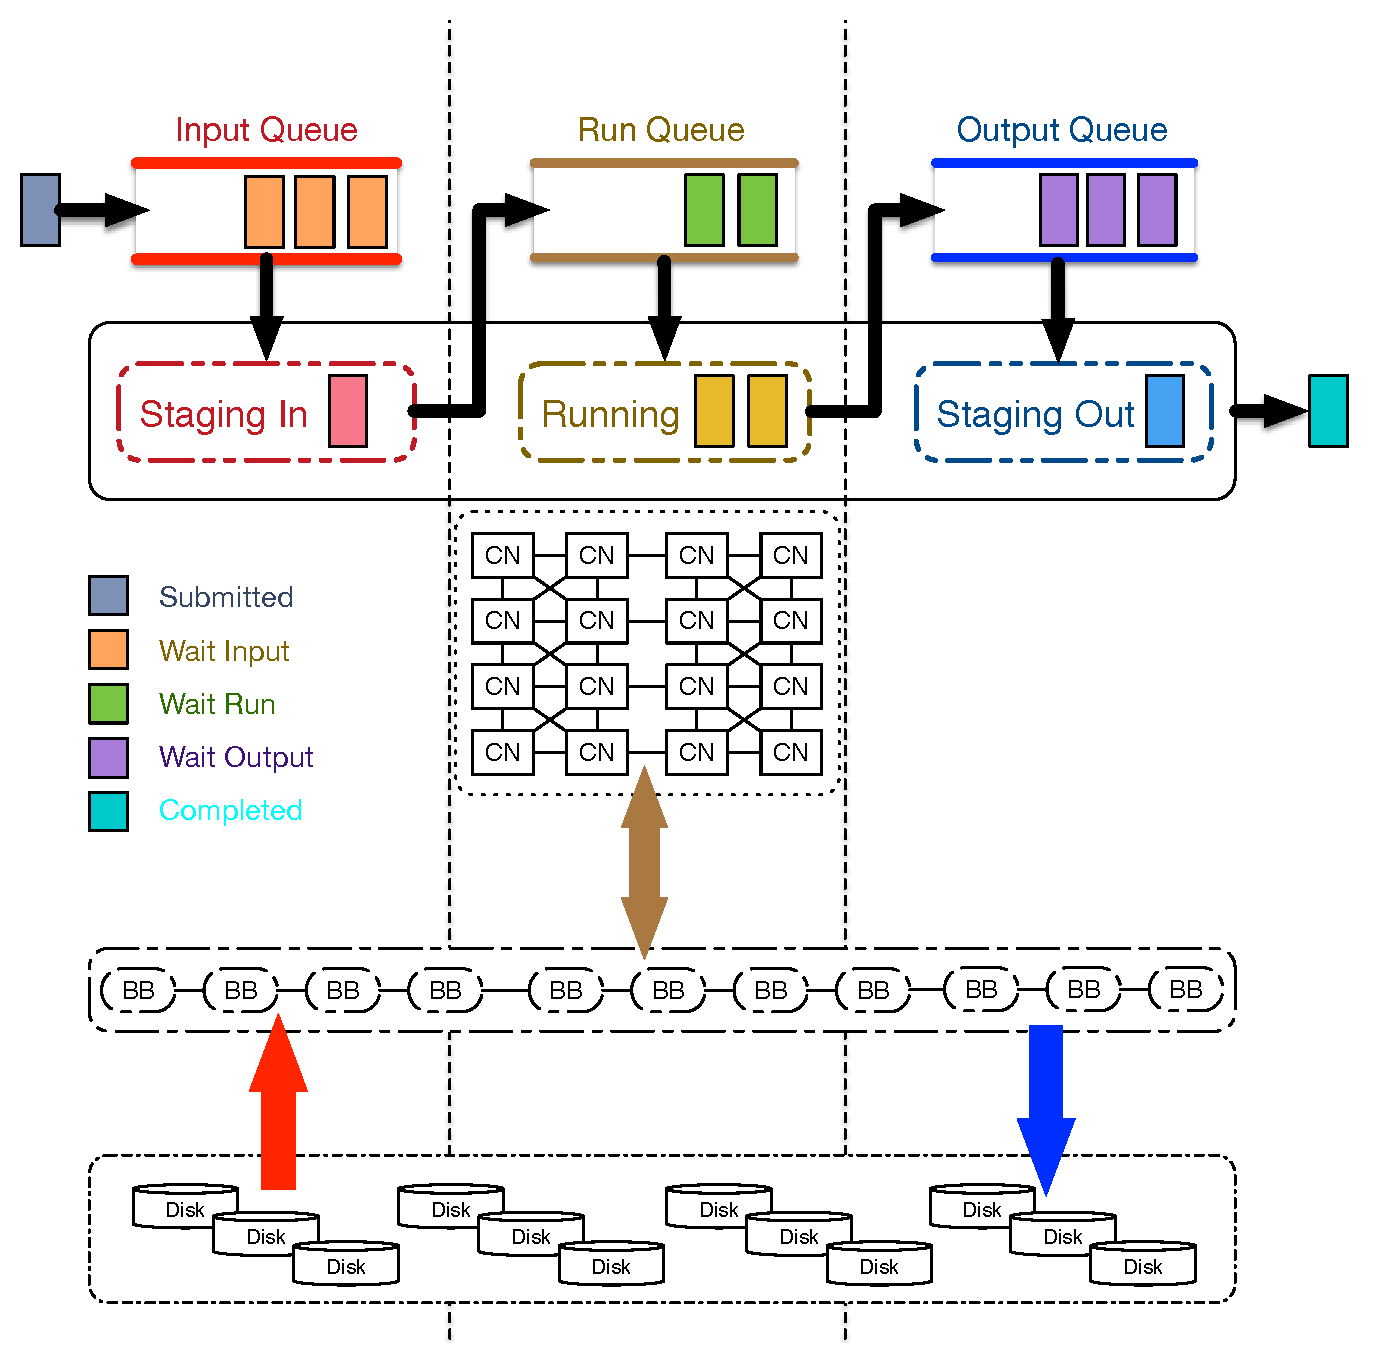
\includegraphics[width=3.6in]{CerberusBBSystem}
        \caption{The design of Three-Phase burst buffer aware scheduling. The black arrows indicate 
        the jobs changing of status; the red, peru and blue arrows in the bottom indicate the data flow in different phases.}
        \label{Fig:CerberusQueues}
\end{figure}

The traditional batch scheduler on a system without burst buffer only considers
the job with the number of required nodes and the expected runtime for the scheduling decision making process.
The most commonly used scheduling policy is the First Come First Serve with EASY backfilling~\cite{tsafrir-tpds-2007}.
However, on burst-buffer-enabled systems,
the amount of available burst buffer capacity becomes a new scheduling constraint.

In this work,
we propose Cerberus, a burst-buffer-aware batch scheduler.
We assume that upon job submission, 
a user specifies the amount of compute nodes, 
the expected job runtime, 
and the amount of burst buffer needed by his/her job. 
Cerberus makes scheduling decisions based on the most common use cases of burst buffer:
data stage-in, checkpointing, and data drain-out.
Cerberus can allocate burst buffer to each job with regard to its use cases
by maintaining three distinct queues, as shown in Figure~\ref{Fig:CerberusQueues}.
The input queue $Q_I$ contains all the jobs that need to prefetch data from the external storage to the burst buffer.
The running queue $Q_R$ holds the jobs that are waiting for the compute nodes and the burst buffer used for checkpointing.
Jobs waiting to be drained out to the external permanent storage are in the output queue $Q_O$.
The layered hierarchy in Figure~\ref{Fig:CerberusQueues} also indicates that burst buffer
can fill in the memory gap between the memory on compute nodes and the hard disk storage.
Cerberus coordinates among three queues and makes scheduling decisions according to job requirements in each queue with the objective to maximize job performance and system utilization.

Before we give the details of our Cerberus design, 
in this section we describe our three-phase job model 
and the corresponding resource demand at each phase. 

%The batch scheduler makes scheduling decisions for 
%each job based on its demand while attempting to
%minimize the overall job response time and maximize the system throughput.
%However, jobs requiring more than one resource could result in possible deadlocks and starvation.
%In order to improve the overall resource utilization and the system responsiveness, we propose
%a fine granularity job model based on the possible use cases of burst buffer.
%In our scheduling framework, the system resources include compute nodes and burst buffer.
%The job resource demand varies in different execution phases;
%Correspondingly, the batch scheduler makes scheduling decisions in each phase.


% Users request the system to run their applications as jobs.
% We define $J = (job_1, job_2, \ldots, job_n)$ to be the set of all unfinished jobs in the system.
% To fully utilizing burst buffer, we divide jobs into 3 different phases.
% In the first phases, input data are staged in from IO nodes to burst buffer.
% We refer this phase as \textit{stage-in} phase.
% It is very easy for user to provide the amount of input data
% because they should already be available before application execution. 
% Then the job can run on the compute nodes after being scheduled;
% except reading data from burst buffer, there may be interaction between 
% computer node and burst buffer.
% These interactions are mainly due to fault tolerance reasons, like check-pointing.
% This phase is called \textit{running} phase.
% When computation is done, output data needs to be staged out to external PFS from memory,
% namely \textit{stage-out} phase.
% Burst buffer plays as an efficient IO broker for compute nodes,
% in replacing of traditional IO nodes.


%=============Xu======================
%\subsection{Three-Phase Job Model}

%Applications can benefit from burst buffer in three major ways\cite{BBUseCase}.
%Before execution, job pre-fetch data from the external storage to the burst buffer.
%When jobs start running on the compute nodes,
%they could burst the checkpoint data to the burst buffer at high speed.
%Upon the job completion, 
%useful output data are staged out to the burst buffer for early releasing the compute nodes.
%Therefore, we divide the job lifetime into three different phases, as illustrated in Figure~\ref{Fig:CerberusQueues}. \NOTE{I prefer we keep this paragraph. Because it explains why 3-Phase make sense. 3-Phase is based on app's use case of bb.}

 
\textbf{Stage-In}: After submitting the job to the system,
         Cerberus needs to prefetch data, such as configuration files and input data,
         from IO nodes to the burst buffer. We define this phase as \textit{stage-in}.
         The only resource needed by the job in this phase is the burst buffer.
         Users are encouraged to specify the amount of burst buffer required in the \textit{stage-in} phase.
         The job is ready to run when the data is prefetched into the burst buffer.
 
\textbf{Running}: The scheduler allocates the job with the required
         number of compute nodes and the amount of burst buffer. 
         It then dispatches the job to the system for running.
         This is defined as \textit{running} phase.
         During the running phase, there could be frequent data exchange
         between the compute nodes and the burst buffer.
         These interactions, such as like check-pointing, are mainly for achieving system fault tolerance. 
 
\textbf{Stage-out}: When the job finishes computation and
         exits the \textit{running} phase, its output data need to be drained out
         to the external storage from the on-node memory. We define this as \textit{stage-out} phase.
         The job can release its compute nodes when the output data are staged out
         into the burst buffer at high speed. The burst buffer serves as an efficient
         IO broker for the compute nodes and drains the output data to the external storage.

%While burst buffer has been utilized during all three phases,
%compute nodes are only required during the \textit{running} phase. 


%\subsection{Three-Phase Resource Demand Model}
% Users typically provide their resource demand for their jobs.
% This is the most important information scheduler could get from the users.
% Therefore, each job is associated with a demand vector in the form of $(c, rt)$
% where $c$ is the number of needed compute node in running phase,
% $rt$ is the requested runtime user can provide to help scheduler make decisions.
% To be burst buffer aware, demand vector should be augmented
% with fields defining user's request for burst buffer capacity.
% We consider two possible ways to do so.
% Corresponding to the typical usage cases of burst buffer,
% user may provide a \textit{burst buffer triple} in the form of $(bb\_in, bb\_run, bb\_out)$,
% where $bb\_in$ is the volume of burst buffer user predicted for staging in data files,
% $bb\_run$ is the volume of burst buffer user preferred for checkpointing during running,
% $bb\_out$ is the volume of burst buffer needed to hold the resulting output data.
% A job that providing demand vector augmented with
% burst buffer triple is called a \textit{3-phase modeled job}.
% Alternatively, a lazy user may just use the $\max\{bb\_in, bb\_run, bb\_out\}$ at every stage.
% %We do not make any assumption about $bb\_run$ and $bb\_out$
% %because it is nontrivial to predict them, both for system scheduler and application owner.
% We refer this augmentation as
% \textit{1-phase modeled jobs} thereafter.

%=========XY===============
Jobs are submitted to the system with the specified resource demand.
Each job is associated with a demand vector in the form of $(c, ert)$,
where $c$ is the number of needed compute nodes in the running phase,
$ert$ is the expected runtime.
In a burst-buffer-enabled system, the demand vector should be augmented
with fields defining user's requests on the burst buffer capacity.
We consider two possible ways that users provide the burst buffer demand.
For the users with accurate speculation about their job's burst buffer demand in each phase,
they may provide a \textit{burst buffer triple} in the form of $(bb\_in, bb\_run, bb\_out)$,
where $bb\_in$ is the volume of burst buffer for staging in data files,
$bb\_run$ is for checkpointing during the execution, and
$bb\_out$ is for staging out the output data.
% A job that providing demand vector augmented with
% burst buffer triple is called a \textit{3-phase modeled job}.
We will show the benefits of providing the job burst buffer demand in the form of \textit{burst buffer triple} in the next section.
Alternatively, a user may just use the $\max\{bb\_in, bb\_run, bb\_out\}$
as the job's burst buffer demand in the whole lifetime.
% We refer this augmentation as
% \textit{1-phase modeled jobs} thereafter.

% The tightly coupling between processing cores and memory makes 3-phase model
% more complicated than it appears in terms of resource releasing.
% For a job at the stage-in phase, compute nodes is not allocated to it yet
% but that will not effect staging in data.
% When scheduler allocate compute nodes (coupled with memory) to a job,
% these nodes are exclusively used by this job.
% The first thing to do in running phase is fetching in data from burst buffer to memory,
% which is not available until compute nodes is allocated to job.
% We refer this sub-phase as \textit{fectch-in} phase.
% $bb\_in$ will be hold by job until \textit{fetch-in} phase finished.
% Even if the computation is done when job exit \textit{running phase},
% compute nodes cannot be released until job enters \textit{stage-out} phase 
% \textbf{and} output data are drained out to burst buffer from memory,
% referred as \textit{drain-out} phase.
% However, $bb\_run$ can be immediately reclaimed at the end of \textit{running phase}.
% Once \textit{drain-out} phase is done,
% compute nodes become available for jobs waiting to be run
% because staging output data out to IO node is the business of burst buffer nodes,
% sometimes with the help from traditional IO nodes.
% Burst buffer nodes used for caching output data can thus be put back for reuse
% when \textit{stage-out} phase, as well as the entire lifetime of job, concludes.



%The resource releasing for the 3-phase modeled jobs is nontrivial. 
%For a job at \textit{stage-in} phase, compute nodes is not allocated to it yet. 
%The job can stage in data from external storage to burst buffer without the involvement of compute nodes.
%When scheduler allocates compute nodes to the job, the job enters the \textit{running} phase 
%and starts to read the pre-fetched data from burst buffer into the main memory, 
%$bb\_in$ will be released after all the data are moved into main memory. 
%When the job finishes computation and exits \textit{running} phase, 
%$bb\_run$ are released while compute nodes are still hold by the job. 
%The compute nodes will be released after all the output data are moved into $bb\_out$ from main memory.
%The job at \textit{stage-out} phase only holds $bb\_out$ burst buffer. 
%Once all the output data are drained out to the external storage,  
%$bb\_out$ is released.


\begin{table}[ht] 
        \renewcommand{\arraystretch}{1.3}
        \caption{Summary of Symbols}
        \label{Tab:Symbols}
        \centering
        \begin{tabular}{l|l}
                \hline
                $CN$ & number of total compute nodes \\
                $BB$ & amount of total burst buffer nodes \\
                $CN_{available}$ & number of available compute nodes \\
                $BB_{available}$ & amount of available burst buffer nodes \\
                $c_i$ & compute node demand of $job_i$ \\
                $bb\_in_i$ & burst buffer demand of $job_i$ at \textit{stage-in} phase \\
                $bb\_run_i$ & burst buffer demand of $job_i$ at \textit{running} phase \\
                $bb\_out_i$ & burst buffer demand of $job_i$ at \textit{stage-out} phase \\
                $rt_i$ & running time of $job_i$ recorded in the log trace \\
                $ert_i$ & estimated or expected running time of $job_i$ \\
                $Q_I, Q_R, Q_O$ & queues for \textit{stage-in, running, stage-out} phases \\
                $J_{Q_I}, J_{Q_R}, J_{Q_O}$ & set of jobs in corresponding queues \\
                $\mathcal{J}_{Q_I}, \mathcal{J}_{Q_R}, \mathcal{J}_{Q_O}$ & selected jobs from the corresponding queues\\
                $p_i$ & profit of $job_i \in J_{Q_R}$ \\
                $dp(\cdot)$ & memo used in dynamic programming \\
                \hline
        \end{tabular}
\end{table}



% \section{Event-driven Burst Buffer Simulator}
% \label{Sec:Simulation}

% We develop an event-driven simulator for burst buffer enabled HPC system, named \textbf{BBSim},
% from scratch in Python to mimic Cerberus scheduling Trinity.\NOTE{Fig has no info about Trinity}
% It roughly consists of 1,400 lines of code.
% Figure~\ref{Fig:JobFSM} illustrates the simulation lifetime of a job in BBSim
% using extended finite state machine (EFSM).
% The \textit{state} of the job changes depending on current status and
% happening \textit{events}, along with which an \textit{action} is taken.
% For example, at the very beginning, submitted $job_i$ will enter \textbf{Waiting Stage-in} state;
% at the meanwhile, $job_i$ is enqueued to $Q_I$ and scheduler is triggered to do scheduling.

%=========XY===========
\section{BBSim for Cerberus}
\label{Sec:Simulation}

We develop an event-driven simulator, named \textbf{BBSim},
to simulate Cerberus scheduling jobs on the burst buffer enabled HPC system.
Aside from demonstrating the lifetime of a job scheduled by Cerberus, 
Figure~\ref{Fig:JobFSM} also illustrates the various events in BBSim and how to handle
them in a event-driven-simulation approach.
The \textit{state} of the job changes depending on current status and
happening \textit{events}, along with triggered \textit{action}.
For example, when $job_i$ is submitted to the system, 
it enters \textit{Waiting Stage-in} state, 
waiting to be scheduled in job queue $Q_I$. 
The scheduler checks $job_i$'s resource demand and 
dispatches it to run when enough resources become available.


% Whenever job enters one of its 3 phases, system resources are allocated:
% \begin{itemize}
%         \item $BB_{in}$ TB amount of burst buffer are allocated upon entering stage-in phase.
%         \item $CN$ number of compute nodes and $BB_{run}$ amount of burst buffer
%                 are allocated upon entering running phase.
%         \item $BB_{out}$ TB of burst buffer are allocated upon entering stage-out phase.
% \end{itemize}
% Various \texttt{release()} actions are of importance because, in addition to submission,
% \texttt{schedule()} is invoked to schedule waiting jobs
% whenever system resources are released:
% \begin{itemize}
%         \item When job's data is loaded from burst buffer to memory,
%                 burst buffer allocated at stage-in phase are released.
%         \item When job finishes running, system reclaims burst buffer nodes
%                 used for checkpointing.
%         \item When job's data is written to burst buffer from memory,
%                 compute nodes taken by job are returned.
%         \item When job's data is staged out to external disk,
%                 its burst buffer nodes are released.
% \end{itemize}
% 
% \begin{figure}[!t]
% \centering
%         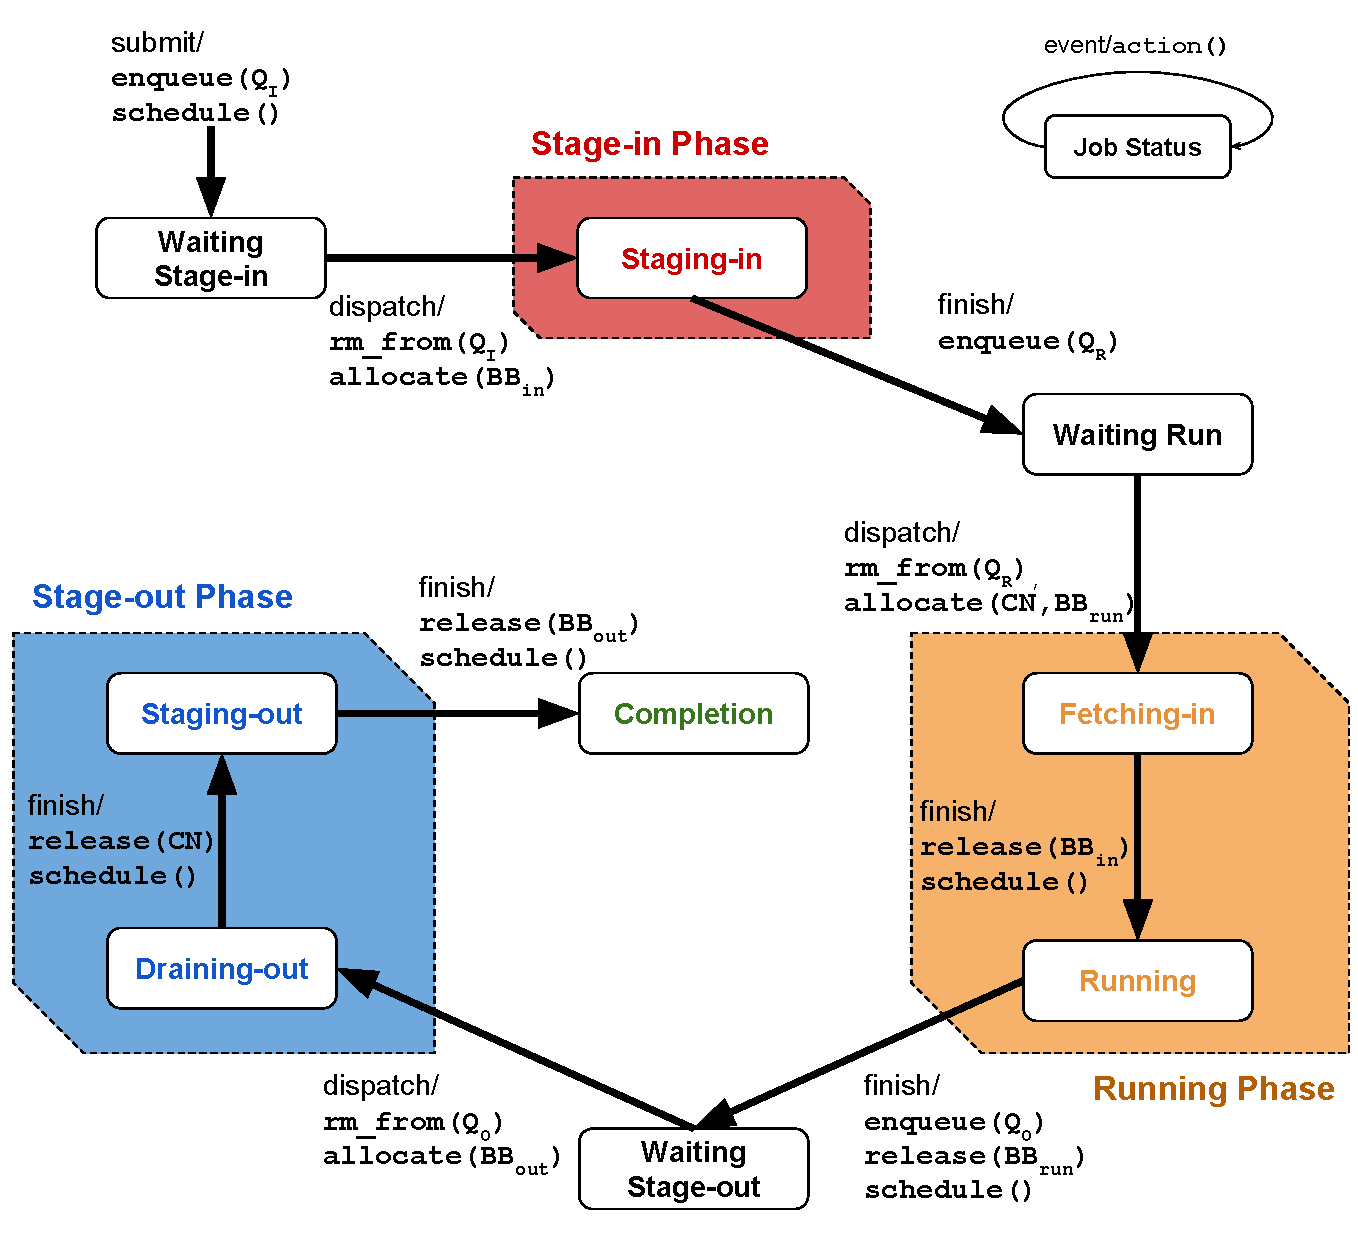
\includegraphics[width=3.6in]{3PhaseJobFSM}
%         \caption{Finite State Machine of Scheduling Simulation}
% \label{Fig:JobFSM}
% \end{figure}


Whenever $job_i$ enters one of the three phases, 
system resources are allocated in the following way:
\begin{itemize}
        \item $BB_{in}$ TB amount of burst buffer are allocated upon entering stage-in phase.
        \item $CN$ number of compute nodes and $BB_{run}$ amount of burst buffer
                are allocated upon entering running phase.
        \item $BB_{out}$ TB of burst buffer are allocated upon entering stage-out phase.
\end{itemize}
Various \texttt{release()} actions are of importance because, in addition to submission,
\texttt{schedule()} is invoked to schedule waiting jobs.
The allocated resource can only be released when certain phase is finished. 
Therefore, any \textit{dispatch} event, generated by \texttt{schedule()} action, 
follows right after a certain \textit{finish} event.
The allocated resources are released at the following time points:
\begin{itemize}
        \item When $job_i$ pre-fetched data from burst buffer to memory,
                burst buffer allocated in stage-in phase ($BB_{in}$) is released.
        \item When $job_i$ finishes computation, 
                system reclaims burst buffer allocated in running phase ($BB_{run}$). 
        \item When $job_i$ output data is written to burst buffer from memory,
              compute nodes ($CN$) allocated in running phase are released
        \item When output data is drained out to external storage,
                burst buffer allocated in stage-out phase ($BB_{out}$) is released.
                Simulation for $job_i$ completes.
\end{itemize}




% Notice that resource can only be released when certain phase is finished.
% Therefore, any \textit{dispatch} event, caused by \texttt{schedule()} action, actually happens
% at the meanwhile of a certain \textit{finish} event.
% The timestamps of all possible \textit{finish} events are calculated in the following way:
% \begin{align}
%         & TS_{f\_stagein} = TS_{s\_stagein} + \frac{bb\_in}{BW_{io\_to\_bb}}\label{Equ:FinIn} \\
%         & TS_{f\_loadin} = TS_{s\_run} + \frac{bb\_in}{BW_{bb\_to\_cn}}\label{Equ:FinMemIn} \\
%         & TS_{f\_run} = TS_{f\_loadin} + \frac{bb\_run}{BW_{cn\_to\_bb}} + rt\label{Equ:FinRun} \\
%         & TS_{f\_loadout} = TS_{s\_stageout} + \frac{bb\_out}{BW_{cn\_to\_bb}}\label{Equ:FinMemOut} \\
%         & TS_{f\_stageout} = TS_{f\_loadout} + \frac{bb\_out}{BW_{bb\_to\_io}} \label{Equ:FinOut}
% \end{align}
% where $TS_{f\_x}$ stands for the timestamps of finishing phase $x$,
% $TS_{s\_x}$ stands for the timestamps of starting phase $x$,
% $BW_{x\_to\_y}$ stands for the bandwidth between $x$ and $y$.
% 
% Though target on burst buffer system, BBSim also supports simulating non-BB HPC system.
% Besides, it is not coupled with Cerberus but easy to simulating many other scheduler.
% Both can be proved by the following experiments for various schedulers.


%==========XY============

The timestamps of all possible \textit{finish} events are calculated in the following way:
\begin{align}
        & TS_{f\_stagein} = TS_{s\_stagein} + \frac{bb\_in}{BW_{io\_to\_bb}}\label{Equ:FinIn} \\
        & TS_{f\_loadin} = TS_{s\_run} + \frac{bb\_in}{BW_{bb\_to\_cn}}\label{Equ:FinMemIn} \\
        & TS_{f\_run} = TS_{f\_loadin} + \frac{bb\_run}{BW_{cn\_to\_bb}} + rt\label{Equ:FinRun} \\
        & TS_{f\_loadout} = TS_{s\_stageout} + \frac{bb\_out}{BW_{cn\_to\_bb}}\label{Equ:FinMemOut} \\
        & TS_{f\_stageout} = TS_{f\_loadout} + \frac{bb\_out}{BW_{bb\_to\_io}} \label{Equ:FinOut}
\end{align}
where $TS_{f\_x}$ stands for the timestamps of finishing phase $x$,
$TS_{s\_x}$ stands for the timestamps of starting phase $x$,
$BW_{x\_to\_y}$ stands for the bandwidth between $x$ and $y$.
BBSim does not simulate the data transfer between IO nodes and PFS through network.
Though targeting on burst buffer enabled systems,
BBSim also supports simulating job scheduling on HPC systems without burst buffer.
Besides, it is easy to integrate any scheduling policies into BBsim.



\section{Cerberus and Optimization Enhancement}
\label{Sec:Scheduler}

\subsection{Cerberus for 3-Phase Jobs}
Traditional batch scheduler usually looks at the field of $c_i$ and $rt_i$
when making scheduling decision.
One straightforward way to make decisions on non-burst-buffer HPC system is
First Come First Serve, as long as available compute nodes can satisfy user job.
Once the system is equipped with burst buffer, scheduler must consider a new constraint:
the available amount of burst buffer capacity.
Scheduling is divided into 3 phases to
adopt to the 3-phase characteristic of jobs in burst buffer context.
As shown in Figure~\ref{Fig:CerberusQueues},
Cerberus schedules jobs in 3 distinct set/queue.
The input queue $Q_I$ contains all the jobs that
needs to load input data before they are able to execute.
Once a job comes out of input queue, its data flows from external disk
to burst buffer nodes, indicated by the red arrow.
Compute nodes are not allocated to the application until
data flows from burst buffer to memory on compute nodes.
The run queue $Q_R$ contains all the jobs waiting to be run with loaded data.
Before executing, input data must be transfered to memory on compute nodes,
after which burst buffer used for stage-in can be released.
When running application request checkpointing, its execution and data are
pushed to its exclusive burst buffer nodes;
when application resume from system fault, its checkpointing are
loaded directly from burst buffer, instead of PFS, to compute nodes.
The output queue $Q_O$ contains all the jobs that
terminate execution but needs to write output data to external storage.
As soon as output data is moved from memory to burst buffer nodes allocated for stage-out,
compute nodes can be released;
in other words, other applications ready to run can take up them now.
At anytime, a job can only appear in one of the 3 sets, apparently.
This fact motivates separated scheduling idiom to be used in different phases,
or for different job queues.

%\begin{figure}[!t]
        %\centering
        %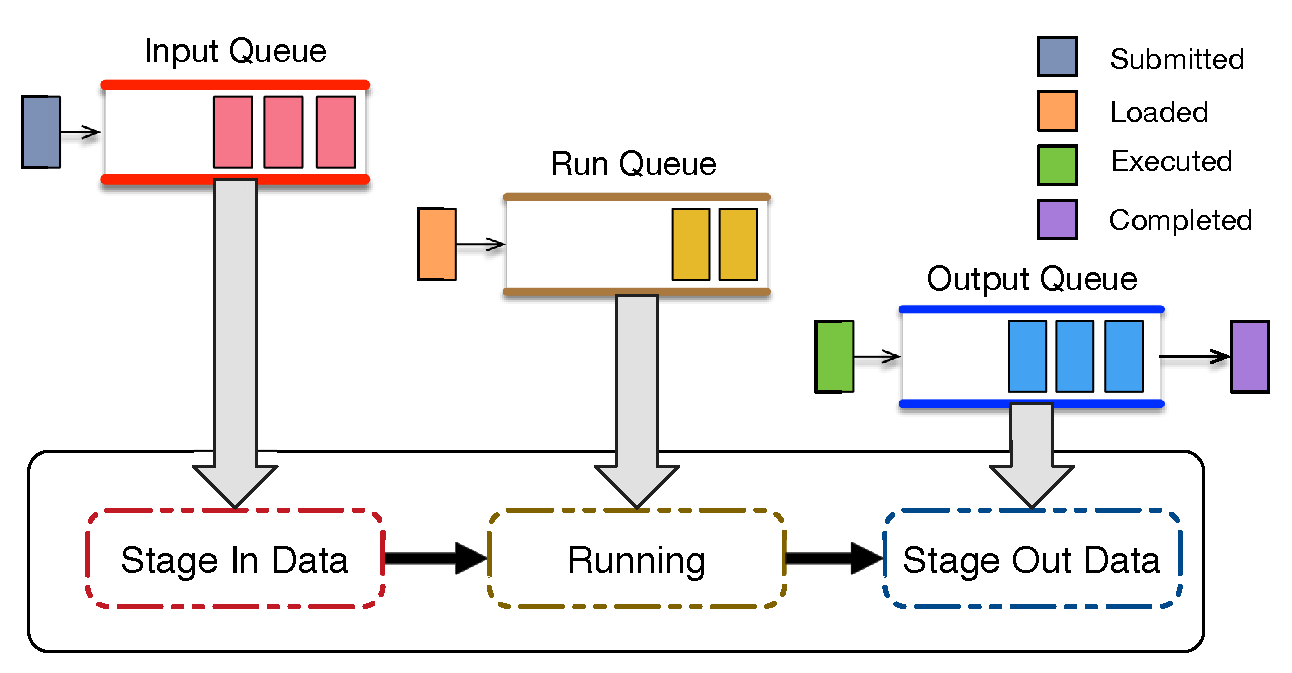
\includegraphics[width=3.6in]{CerberusQueues}
        %\caption{Scheduling Process of Burst Buffer Aware Cerberus}
        %\label{Fig:CerberusQueues}
%\end{figure}

\begin{figure}[!t]
        \centering
        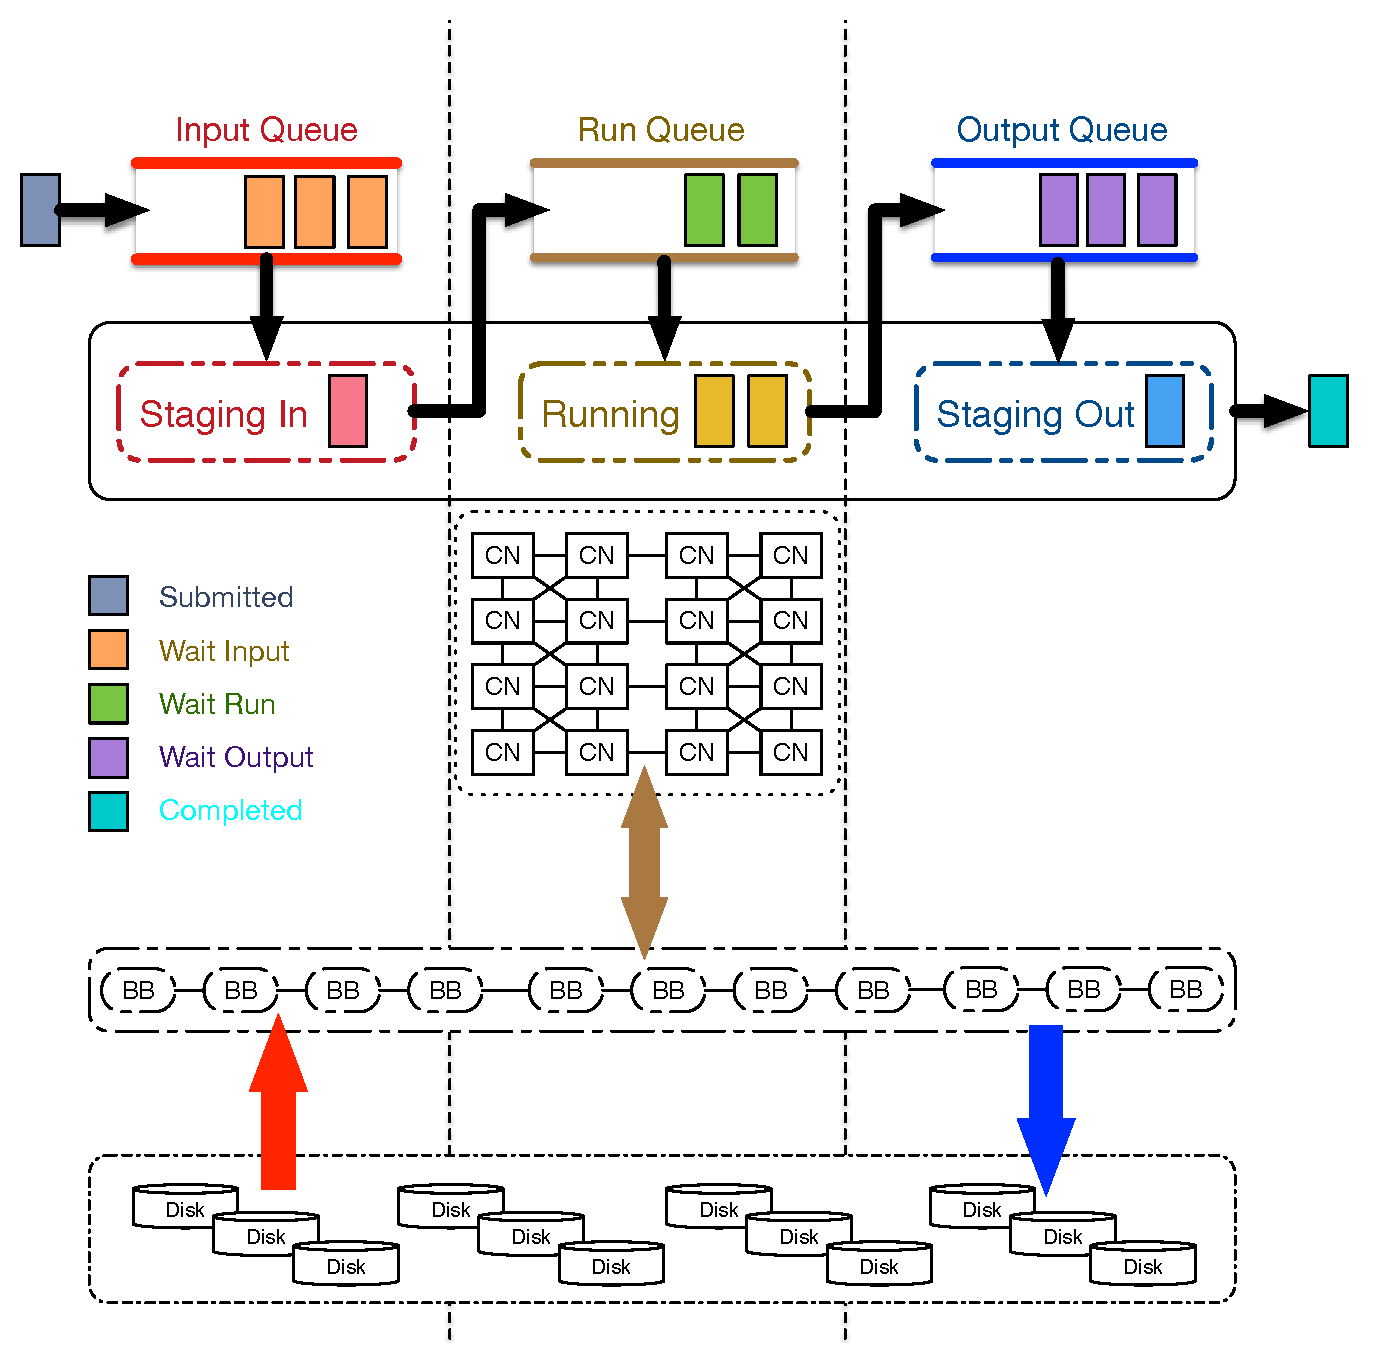
\includegraphics[width=3.6in]{CerberusBBSystem}
        \caption{Scheduling Workflow of Burst Buffer Aware Cerberus}
        \label{Fig:CerberusQueues}
\end{figure}


\subsection{Optimize Stage-In Phase}
In the stage-in phase, only burst buffer demand is considered.
Scheduling is made based on the value of $bb\_in$ of jobs in $Q_I$.
If we care about data transfer throughput,
we should transfer as much data as possible by doing the following optimization:
\begin{align*}
        & \max \sum_{i\in S} bb\_in_i \\
        & s.t. \sum_{i\in S} bb\_in_i \leq BB_{available} \numberthis \label{Equ:MaxTransferData}
        %\left\{
                %\begin{array}{l}
                        %S \subseteq J_{Q_I} \\ [1em]
                        %\sum_{i\in S} bb\_in_i \leq BB_{available}
                %\end{array} 
        %\right.
\end{align*}
where $J_{Q_I}$ stands for all jobs in input queue at the time considering,
$S\subseteq J_{Q_I}$ is the set of job selected by Cerberus,
$bb\_in_i$ is the burst buffer demand of $job_i$,
$BB_{available}$ is system's available amount of burst buffer.

If we care about task parallelism, following optimization could help:
\begin{align*}
        & \max |S| \\
        & s.t. \sum_{i\in S} bb\_in_i \leq BB_{available} \numberthis \label{Equ:MaxTaskNumber}  
        %\left\{
                %\begin{array}{l}
                        %S \subseteq J_{Q_I} \\ [1em] 
                        %\sum_{i\in S} bb\_in_i \leq BB_{available}
                %\end{array} 
        %\right.
\end{align*}
The number of tasks doing data loading will be maximized.


\subsection{Optimize Running Phase}
Running jobs require not only compute nodes, but burst buffer to ensure performance and correctness.
Scheduling are accordingly made based on the value of $c$ and $bb\_run$ of jobs in $Q_R$.
To maximize multiple types of resource's utilization,
we convert it to the knapsack problem by defining the value of the $job_i$ as
\begin{equation}
        v_i = \frac{c_i / CN}{rt_i} \times \frac{bb\_run_i / BB}{rt_i}
        \label{Equ:DefValue}
\end{equation}
where $rt_i$ is the running time of $job_i$, the time it takes up the computing nodes.
By defining \textit{value} as Equation~\ref{Equ:DefValue},
we prefer these tasks that claims to take up node resources with short duration.
Unfortunately, it is difficult to predict $rt_i$ before actually running the job.
Of course we could use the \textit{expected running time} $ert_i$ specified by user.
However, by examining the log traces from Argonne National Laboratory (ANL)\cite{JobTrace},
we found that the variance between $rt_i$ and $ert_i$ is significantly different.
For now we can just assume $ert_i$ represent $rt_i$ of $job_i$.
In the future, we could adopt machine learning or data mining ideas
to predict the running time of a job with demand vector.
%Notice that then the value of a task is proportional to $c_i*bb_i$.
The optimizing formula can thus be
\begin{align*}
        & \max \sum_{i \in S}\frac{c_i}{ert_i} * \frac{bb\_run_i}{ert_i} \\
        & s.t. \left\{
                \begin{array}{l}
                        %S \subseteq J_{Q_R} \\ [1em]
                        \sum_{i \in S} c_i \leq CN_{available} \\ [0.5em]\numberthis \label{Equ:MaxProduct} 
                        \sum_{i \in S} bb\_run_i \leq BB_{available}
                \end{array} 
        \right.
\end{align*}
where $J_{Q_R}$ is the set of jobs in running queue,
$S\subseteq J_{Q_R}$ stands for jobs selected by scheduler,
$CN_{available}$ and $BB_{available}$ represent the amount of system's available resources
(compute nodes and burst buffer nodes) at current moment.

\subsection{Optimize Stage-Out Phase}
Scheduling are made based on the value of $bb\_out$ of jobs in $Q_O$.
Optimization formula for different purpose are almost the same as
Equation~\ref{Equ:MaxTransferData} and Equation~\ref{Equ:MaxTaskNumber}
in stage-in scheduling, except that $bb\_in$ is replaced with $bb\_out$,
$J_{Q_I}$ is replaced with $J_{Q_O}$, the job set of output queue.


\subsection{Solving the Optimization Problems}
It is trivial to show that optimization problem~\ref{Equ:MaxTransferData}
and~\ref{Equ:MaxTaskNumber}
are equivalent to 0-1 knapsack problem.
Problem~\ref{Equ:MaxProduct} can be informally treat as 2-dimension 0-1 knapsack problem.
In fact, we expect all of them are NP-hard problems.
We can solve them with dynamic programming in pseudo polynomial time.
Applying memorization could also help accelerate the solving process.
In fact we are not interested in the optimal result of problem~\ref{Equ:MaxTransferData},
problem~\ref{Equ:MaxTaskNumber} and problem~\ref{Equ:MaxProduct} at all
but in a combination of jobs that yields the optimal solution,
which can also be easily tracked back down by keeping memorizations.

%The solution to Problem~\ref{Equ:MaxTransferData},
%Problem~\ref{Equ:MaxTaskNumber} and Problem~\ref{Equ:MaxProduct} are similar.
First, for Problem~\ref{Equ:MaxTransferData}, the recursive relationship is
given by Recursion~\ref{Equ:MaxTransferDataRecursion}.
In~\ref{Equ:MaxTransferDataRecursion}, the memo we keeps during solving is
the optimal solution for 
$jobs=(job_1, job_2, \ldots, job_i)$ with $w$ GB of available burst buffer.
It turns out that the recursion for Problem~\ref{Equ:MaxTaskNumber} is
extremely similar to~\ref{Equ:MaxTransferDataRecursion}
The memo in Recursion~\ref{Equ:MaxTaskNumberRecursion} is the same
as that in Recursion~\ref{Equ:MaxTransferDataRecursion}.
The recursion for Problem~\ref{Equ:MaxProduct} is a little bit complicated.
Here we should keep the memo of the optimal solution for $jobs=(job_1, job_2, \ldots, job_i)$
with $c$ computing nodes and $w$ GB of burst buffer being available.

Scheduler can obtain an optimal combination of jobs by examining the memo.
Take the problem~\ref{Equ:MaxProduct} problem for example.
We start from $dp(n, CN, BB)$.
If $c_n \leq CN$ and $bb\_in_n \leq BB$, $job_n$ should be scheduled if
$dp(i-1, c, w) \leq dp(i-1, c - c_i, w - bb\_in_i) + c_i bb\_in_i$ and
recurse with $dp(n - 1, CN - c_i, BB - bb\_in_i)$;
otherwise, $job_n$ should be skipped and we recurse the process on $dp(n-1, CN, BB)$.
The time complexity of solving Equation~\ref{Equ:MaxTransferDataRecursion} and
Equation~\ref{Equ:MaxTaskNumberRecursion} is $O(n\times BB)$.
The time complexity of solving Recursion~\ref{Equ:MaxProductRecursion}
is $O(n\times CN\times BB)$.
Notice that $CN$ and $BB$ may be very large integers,
making the pseudo-polynomial algorithm unsuitable
to be used online by scheduler.
In practice, we could reduce the time complexity by allocating resource
in a coarser granularity.
For example, jobs usually asks for compute node in the unit of $cn\_unit = 512$ nodes;
their demands for burst buffer nodes are usually in the unit of $bb\_unit = 100$ GB.
We can divide both $CN$ and $c_i$ by $cn\_unit$;
divide both $BB$ and $bb\_in, bb\_run, bb\_out$ by $bb\_unit$.
It is also possible to reduce the value of $n$, the number of jobs in the queue.
For example, we can consider only $\frac{1}{\alpha}n$ jobs in the queue.
This will give us only the partial optimal solution
in exchange of less computation complexity.

\begin{strip}
        \begin{align}
                dp(i, w) = & 
                \left\{
                        \begin{array}{l}
                                0, \text{ if $i=0$ } \\ [0.4em]
                                dp(i-1, w), \text{ if $bb\_in_i > w$} \\ [0.4em]
                                \max \{ dp(i-1, w), dp(i-1, w-bb\_in_i) + bb\_in_i \}, \text{ if $bb\_in_i \leq w$}
                        \end{array} 
                \right.
                \label{Equ:MaxTransferDataRecursion} 
        \end{align}
\end{strip}
\begin{strip}
        \begin{align}
                dp(i, w) = &
                \left\{
                        \begin{array}{l}
                                0, \text{ if $i=0$ } \\ [0.4em]
                                dp(i-1, w), \text{ if $bb\_in_i > w$} \\ [0.4em]
                                \max \{ dp(i-1, w), dp(i-1, w-bb\_in_i) + 1 \}, \text{ if $bb\_in_i \leq w$}
                        \end{array} 
                \right.
                \label{Equ:MaxTaskNumberRecursion}
        \end{align}
\end{strip}
\begin{strip}
        \begin{align}
                dp(i, c, w) = &
                \left\{
                        \begin{array}{l}
                                0, \text{ if $i=0$ } \\ [0.4em]
                                dp(i-1, c, w), \text{ if $c_i > c$ or $bb\_run_i > w$} \\ [0.4em]
                                \max \{ dp(i-1, c, w), dp(i-1, c - c_i, w - bb\_run_i) + v_i \}, \text{ if $c_i \leq c$ and $bb\_run_i \leq w$}
                        \end{array} 
                \right.
                \label{Equ:MaxProductRecursion}
        \end{align}
\end{strip}



\section{Experiments}
\label{Sec:Experiments}

% This section evaluate Cerberus by answering several key questions.
% \begin{itemize}
%         \item \textbf{Q1}: will Cerberus improve application performance
%                 by utilizing burst buffer nodes?
%         \item \textbf{Q2}: Will job demand on burst buffer affect Cerberus?
%                 Why bother to divide the job execution into 3 phases?
%         \item \textbf{Q3}: Can dynamic programming based optimization
%                 help Cerberus further
% improve application performance?
% \end{itemize}
% Our newly developed event-driven simulator, BBSim, is used to simulating
% the Trinity system described later.

%==============XY===================
This section evaluate Cerberus by answering several key questions.
\begin{itemize}
        \item \textbf{Q1}: will utilizing burst buffer nodes could improve both jobs and system performance?
        \item \textbf{Q2}: Will job demand on burst buffer affect Cerberus?
                Why bother to divide the job execution into 3 phases?
        \item \textbf{Q3}: Can dynamic programming based optimization
                makes Cerberus even better?
\end{itemize}
We integrate Cerberus into our newly developed event-driven simulator, 
BBSim, and evaluate Cerberus against the traditional FCFS/EASY backfilling scheduler.
Codebase of BBsim and Cerberus are public to the community
\footnote{Available at https://github.com/urlplaceholder}.
% metric

% We select two evaluation metrics, job's \textit{response time} and 
% \textit{system throughput}, when evaluating our design.
% Response time is the time duration from job submission to its fully completion,
% which is the major concern from user's perspective.
% On the other hands, system throughput, defined as the number of jobs finished in
% a fixed time period (500 seconds), measures the performance of computing system.

%==============XY===================
We select three evaluation metrics, job's \textit{response time}, \textit{wait time} and 
\textit{system throughput}, when evaluating our design.
Response time is the time duration from job submission to its fully completion,
which is the major concern from user's perspective.
Wait time is the aggregated time a job waits in each phase.
System throughput, defined as the number of jobs finished in
a fixed time period (500 seconds), measures the performance of the system.


\subsection{Simulation Settings}
% % system
% We consider simulating the full Trinity super computer\cite{TrinitySystem}.
% The number of compute nodes on Trinity is about 18,936,
% e.g. 9,436 Intel Haswell nodes
% and at least 9500 Intel Xeon Phi nodes.
% There are 16 cores on each processor, thus totally 302,976 cores.
% In the following experiments, we compare two identical system except that
% IO nodes are replaced by the same number of burst buffer nodes.
% Eventually Trinity plans to delivery up to 576 burst buffer nodes of 3.7 PB,
% consisted of Trinity IO nodes with PCIe SSD card.
% They are globally accessible as intermediate storage and distributed among cabinets.
% Sequential read/write speed of burst buffer nodes is 8.0 GBps.
% Bandwidth between CPU node and non-burst-buffer IO node is set to 2.5 GBps.

%==============XY===================
The parameters used in our simulation are inspired and sampled by Trinity~\cite{TrinitySystem}, 
the next generation supercomputer in Los Alamos National Laboratory.
The simulated system consists of 18,936,
e.g. 9,436 Intel Haswell nodes
and at least 9500 Intel Xeon Phi nodes.
There are 576 burst buffer nodes with aggregated 3.7 PB storage capacity, 
which are globally accessible as intermediate storage.
Sequential read/write speed of burst buffer nodes is 8.0 GBps.
Bandwidth between CPU node and non-burst-buffer IO node is set to 2.5 GBps.

% % trace
% Job trace is from ANL's Blue Gene Intrepid system,
% containing totally 68,936 jobs run during January to September 2009\cite{JobTrace}.
% We extract two critical fields from this jobs trace: running time and
% number of cores user requested.
% In this section we take a window of 1,185 jobs and report their scheduling results.
% We patched 3 fields to each job's log entry: the amount of input data $data\_in$,
% the total amount of written data for checkpointings $data\_run$
% and the amount of output data $data\_out$.
% We assume $data\_run$ and $data\_out$ follows uniform distribution with
% lower boundary of 1 TiB and upper boundary of 60 TiB;
% $data\_in$ follows uniform distribution between 1 GiB and 30 Gib.
% The patches 3 fields may or may not be used in scheduling,
% depends on both the model of the jobs and the experiment scenario.


%==============XY===================
Since Trinity is not ready for the time being, there is no Trinity job log available for our study.
We use the job log collected from ANL's Blue Gene Intrepid system. The log contains 68,936 jobs
submitted to the system from January to September 2009~\cite{JobTrace}.
We patched 3 fields to each job's log entry: the amount of input data $data\_in$,
the total amount of written data for checkpointings $data\_run$
and the amount of output data $data\_out$.
We assume $data\_run$ and $data\_out$ follows uniform distribution with
lower boundary of 1 TiB and upper boundary of 60 TiB;
$data\_in$ follows uniform distribution between 1 GiB and 30 Gib.



\subsection{Q1: BB-enabled system vs. Direct-IO system}
\label{Sec:Sim:DirectIOvsBB}
% In this section, we demonstrate that by utilizing burst buffer nodes,
% job scheduler could improve the performance of both applications and system.
% We compare two systems:
% \begin{itemize}
%         \item \textbf{1-Phase IO}: system without burst buffer nodes
%                 scheduled by FCFS policy
%         \item \textbf{Cerberus}: system with burst buffer 
%                 scheduled by our proposed Cerberus
% \end{itemize}


%=============XY==============
In this section, we demonstrate that by utilizing burst buffer nodes,
both the performance of jobs and system can be greatly improved. 
We compare the overall performance on burst buffer enabled system
against the traditional system without burst buffer (Direct IO).


% Figure~\ref{Fig:DirectIOvsBBResponse} compares CDF of the response time of 1185 jobs.
% When scheduler can allocate burst buffer to jobs,
% response time is bounded by 376,443.12 seconds.
% However, the worst case in system without burst buffer
% (Direct IO) is catastrophical.
% There are jobs that takes 889,239.20 seconds to finish,
% which is 2.36 times slow as the most non-responsive job
% in system equipped with burst buffer.
% In average case, \textit{nearly 99\% of the jobs scheduled by Cerberus
% response faster than Direct batch scheduler on non-BB system.}
% The improvement mainly comes from the difference of IO operation efficiency between
% traditional IO nodes and burst buffer nodes.

%=============XY==============
Figure~\ref{Fig:DirectIOvsBBResponse} compares CDF of jobs response
time by on burst buffer enabled system and the traditional system (Direct IO).
When running on system with burst buffer,
jobs response time is bounded by 376,443.12 seconds.
However, the worst case of Direct-IO is catastrophic.
There are jobs that takes 889,239.20 seconds to finish,
which is 2.36 times slow as the most non-responsive job
in system equipped with burst buffer.
In average case, \textit{nearly 99\% of the jobs scheduled on the burst buffer enabled system
response faster than the traditional system without burst buffer.}
The improvement is intuitive, since the burst buffer can mitigate the IO gap between
IO nodes and compute nodes.


% Figure~\ref{Fig:DirectIOvsBBWait} reveals the total waiting time for both cases.
% Notice that system without burst buffer only request compute nodes.
% In this case, waiting time is the duration from its submission
% to actual starting running.
% The difference of worst case waiting time is drastic.
% Without burst buffer nodes, job's wait duration in worst case is 3.02 times
% slow as the worst one on systems with burst buffer;
% the upper bound of waiting duration for burst buffer systems is about 285,254 seconds.
% Because of burst buffer's better ability to
% absorb checkpoint operations and data moving in/out,
% the execution pipeline of job series is significantly speed up.
% Statistically, \textit{more than 80\% jobs waited less time, thus response faster,
% if they can access burst buffer.}

%=============XY==============
Figure~\ref{Fig:DirectIOvsBBWait} reveals jobs aggregated waiting time.
Noticing that in the case of Direct IO, jobs only request compute nodes.
Thus, waiting time is the duration between submission
and starting to run.
The difference of worst case waiting time is drastic.
On the system without burst buffer nodes, job's wait duration in worst case is 3.02 times
slow as the worst one on the burst buffer enabled system;
the upper bound of waiting duration for burst buffer systems is about 285,254 seconds.
Because of burst buffer's better ability to
absorb checkpoint operations and data moving in/out,
the execution pipeline of job series is significantly speed up.
Statistically, \textit{more than 80\% jobs waited less time, thus response faster,
if they can access burst buffer.}

% Using the collected completion time, we calculate system's throughput over time sequence.
% Figure~\ref{Fig:DirectIOvsBBThroughput} shows the system throughput for
% both system using burst buffer nodes and not.
% As indicated by the bar chart,
% \textit{the ratio of average throughput between two systems is 2.36},
% namely 1.575 to 0.667.
% It totally takes 889,239 seconds for the system without burst buffer nodes to
% server all 1185 jobs.
% The last job is job \#1150, which requested 4096 cores and 59 TB data space.
% It starts at 1126 seconds but waited 827,241 seconds.
% In contrast, when system installed burst buffer nodes,
% it accomplishes the same 1185 jobs in 376,443 seconds.
% Job \#1150 is the second last job finished, but both its waiting time and response time
% are significantly reduced, 272,741 and 376,026 seconds respectively.

%=============XY==============
Figure~\ref{Fig:DirectIOvsBBThroughput} shows the system throughput for
both system using burst buffer nodes and not.
As indicated by the bar chart,
\textit{the ratio of average throughput between two systems is 2.36},
namely 1.575 to 0.667.
It totally takes 889,239 seconds for the system without burst buffer nodes to
complete the workload.
We pick a specific job, job with ID \#1150 from the workload, to observe its
waiting time in both cases.
Job \#1150 request 4096 cores and 59 TB data space.
It starts at 1126 seconds but waited 827,241 seconds.
In contrast, when system installed burst buffer nodes,
it accomplishes the same workload in 376,443 seconds, and waiting time and response time of job \#1150
are significantly reduced, 272,741 and 376,026 seconds respectively.
\NOTE{Xu's suggestion: replace the legend in Fig4,5. 1-Phase IO->Direct IO, Cerberus->BB-enabled}


\begin{figure*}[!t]
        \centering
        \subfloat[Job Response Time] {
                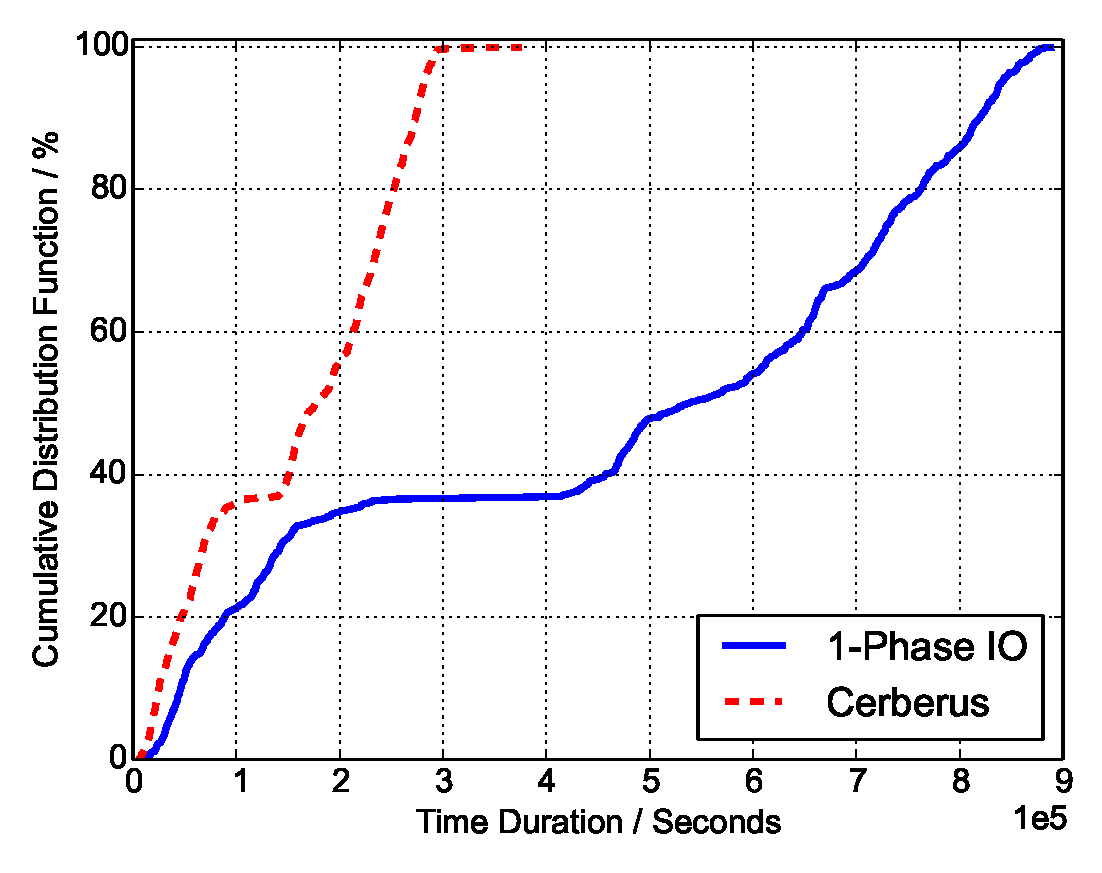
\includegraphics[width=3.2in]{IOvsBBFigures/1000jobs_direct_vs_bb_response}
                \label{Fig:DirectIOvsBBResponse}
        }
        ~
        \subfloat[Job Wait Time] {
                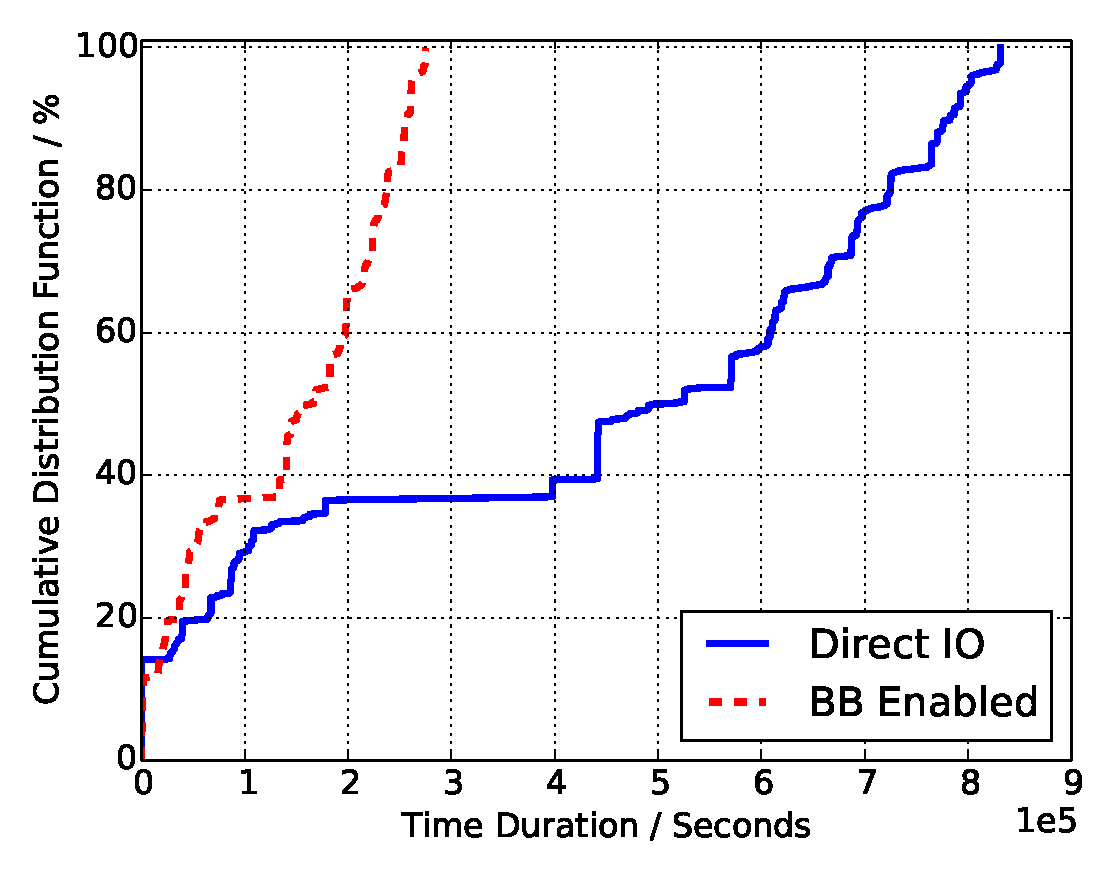
\includegraphics[width=3.2in]{IOvsBBFigures/1000jobs_direct_vs_bb_wait}
                \label{Fig:DirectIOvsBBWait}
        }
        \caption{Jobs Performance: IO Node Only System vs. Burst Buffer System}
        \label{Fig:DirectIOPerformance}
\end{figure*}

\begin{figure}[!t]
        \centering
        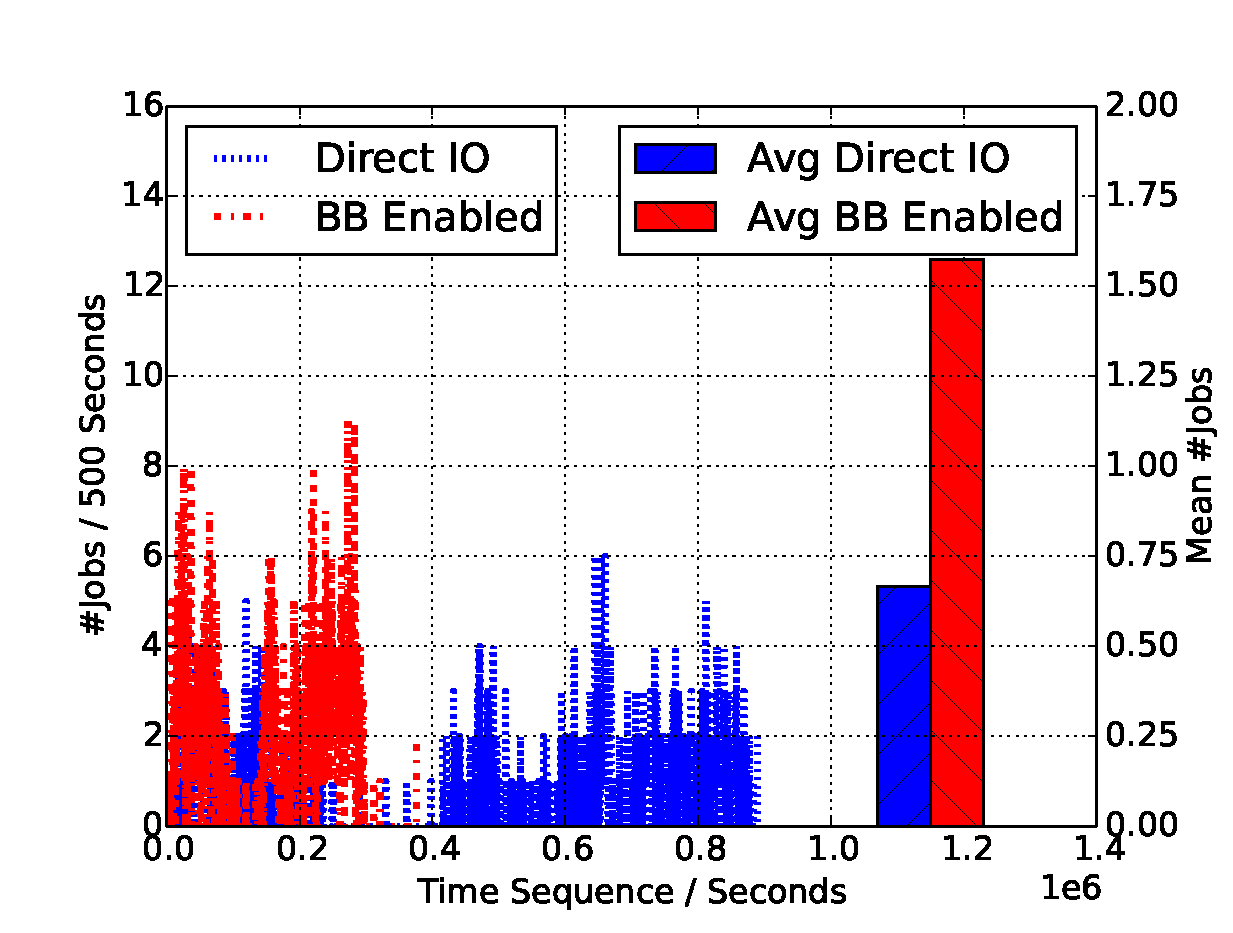
\includegraphics[width=3.2in]{IOvsBBFigures/1000jobs_direct_vs_bb_throughput}
        \caption{System Throughput, IO Node Only vs. Burst Buffer System}
        \label{Fig:DirectIOvsBBThroughput}
\end{figure}


\subsection{Q2: Demand Granularity Matters?}

\NOTE{change terms in this section. The logic is we have three job models. 1-phase-1d, 3-phase-1d, and 3-phase-3d. 
For both 3-phase-1d, and 3-phase-3d, Cerberus is used for job scheduling}

In this section we validate our 3-phase model.
Jobs performance are improved when the scheduler makes scheduling decision in each phase separately.
This encourages user to provide detailed burst buffer demand in each phase for her job.

% In Figure~\ref{Fig:3Pvs1PResponse}, we plot 3 different scheduling results by 3 FCFS scheduler.
% \begin{itemize}
%         \item \textbf{1-Phase BB}: Jobs are modeled as just 1 phase.
%                 Users just provide general burst buffer demand throughout
%                 entire application lifetime.
%         \item \textbf{1D Cerberus}: In this case Cerberus only knows
%                 the overall burst buffer demand.
%         \item \textbf{Cerberus}: Users kindly provided all the burst buffer
%                 demand in all 3 phases.
%                 %the same as Cerberus in section~\ref{Sec:Sim:DirectIOvsBB}
% \end{itemize}
% We simulate the 3 cases with the same generated random data volume sequence.
% We assume the overall burst buffer demand in 1-phase BB and 1D Cerberus is
% $\max \{data\_in, data\_out, data\_run\}$.
% Notice that 1-phase BB scheduler must subject to burst buffer capacity constraint.
% %For 1-phase-modeled jobs, scheduler will make decision
% %based on $\max \{data\_in, data\_out, data\_run\}$
% %since we assume user will only tell the upper bound of its application's demand.
% %However, in simulation, we use the generated data amount as the same as 3-modeled jobs.
% %Response time of system without burst buffer devices are also plotted for comparison.

%========XY========================
In Figure~\ref{Fig:3Pvs1PResponse}, the results of scheduling jobs based on three models
are presented. The three models are:
\begin{itemize}
        \item \textbf{1-Phase-1D}: Jobs are submitted with total burst buffer demand, 
        but their lifetime are not divided into three phases. 
	Instead, the scheduler makes scheduling decision only once for each job.

        \item \textbf{3-Phase-1D}: Jobs are submitted with total burst buffer demand,
        their lifetime are divided into three phases as discussed in section~\ref{Sec:Model}
        
        \item \textbf{3-Phase-3D}: Jobs are submitted with detailed burst buffer demand for each phases.
                %the same as Cerberus in section~\ref{Sec:Sim:DirectIOvsBB}
\end{itemize}
We simulate the 3 cases with the same generated random data volume sequence.
We assume the overall burst buffer demand in 1-Phase-1D and 3-Phase-1D is
$\max \{data\_in, data\_out, data\_run\}$.
Notice that 1-phase BB scheduler must subject to burst buffer capacity constraint.
Cerberus is responsible for scheduling jobs in 3-Phase-1D and 3-Phase-3D model.
The scheduling decision is made for all three models are FCFS based.

% 
% %Unsurprisingly, jobs' response time is improving as long as they could utilizing burst buffer.
% When comparing scheduling results of 1-Phase BB and 1D Cerberus,
% both of which only have rough data information of application,
% more than 60\% of the 3-phase-modeled jobs finish faster than 1-phase-modeled jobs.
% The longest 3-phase-modeled job takes 418,927 seconds to finish
% while the slowest 1-phase-modeled job needs about 492,591 seconds to finish.
% The improvement is about 14.95\% for the worst case.
% The reason of such improvement is as follows.
% For the 1-phase-modeled jobs, burst buffer nodes will be exclusively
% taken by scheduled jobs throughout their lifetime.
% In contrast, Cerberus will reclaim burst buffer multiple times;
% it also releases burst buffer nodes and CPU resources as soon as possible.
% This gives Cerberus more opportunity to schedule the system resources.
% At last, when comparing the case of Cerberus with 1D Cerberus,
% we find another advantage of our 3-phase model.
% If benign users can provide finer-grain information of data/IO demand,
% Cerberus can programme each queue separately and get better scheduling result.
% In our simulation,
% since Cerberus knows more about application's demand in different phases,
% the worst absolute response time is less than 379,026 seconds.
% This is 10.24\% improvement to 3-phase-modeled jobs
% when Cerberus only knows the upper bound of data demand,
% 23.66\% better than the slowest 1-phase-modeled job.
% In average case, \textit{more than 80\% of the jobs 
% scheduled by Cerberus finish earlier than 1-phase-modeled jobs.}
% Meanwhile, \textit{more than 60\% of the jobs takes less time if user 
% specifies data usage demand at each phase to Cerberus, e.g. Cerberus vs. 3-Phase-1D.}


%==============XY===============
When comparing scheduling results of 1-Phase-1D and 3-Phase-1D,
both of which only have overall burst buffer demand of each job,
more than 60\% of the 3-phase-modeled jobs finish faster than 1-phase-modeled jobs.
The longest 3-phase-modeled job takes 418,927 seconds to finish
while the slowest 1-phase-modeled job needs about 492,591 seconds to finish.
The improvement is about 14.95\% for the worst case.
The reason of such improvement is as follows.
For the 1-phase-modeled jobs, burst buffer nodes will be exclusively
taken by scheduled jobs throughout their lifetime.
In contrast, Cerberus will reclaim burst buffer multiple times;
it also releases burst buffer nodes and CPU resources as soon as possible.
This gives Cerberus more opportunity to schedule the system resources.
At last, when comparing the case of 3-Phase-3D with 3-Phase-1D,
we find another advantage of our 3-phase model.
If benign users can provide finer-grain information of data/IO demand,
Cerberus can programme each queue separately and get better scheduling result.
For the 3-Phase-3D model,
Cerberus knows each job's demand in different phases,
the worst absolute response time is less than 379,026 seconds.
This is 10.24\% improvement to 3-phase-modeled jobs
when Cerberus only knows the upper bound of data demand,
23.66\% better than the slowest 1-phase-modeled job.
In average case, \textit{more than 80\% of the jobs 
modeled by 3-phase-3D finish earlier than 1-phase-modeled jobs.}
Meanwhile, \textit{more than 60\% of the jobs takes less time if user 
specifies data usage demand at each phase, e.g. 3-Phase-3D vs. 3-Phase-1D.}



% We can reason about why Cerberus's scheduling result is better than
% naively integrating batch scheduler with burst buffer constraint
% by looking at the detailed waiting time.
% Figure~\ref{Fig:3Pvs1PWaitRun} shows the time job spend in running queue.
% There are 3 queues in Cerberus;
% correspondingly we have 3 kinds of waiting for jobs in Cerberus.
% %Figure~\ref{Fig:3Pvs1PWaitIn} shows the time job spend in inputing queue,
% %Figure~\ref{Fig:3Pvs1PWaitOut} the time job spend in outputing queue.
% For 1-phase-modeled jobs, there is just one queue;
% therefore the waiting time in Figure~\ref{Fig:3Pvs1PWaitRun} is the total waiting time.
% We see that jobs did not spend much time in either input queue $Q_I$ or output queue.
% The upper bounds of time spent in input queue are
% 2500 seconds for 1D Cerberus and Cerberus respectively.
% This is because input data is very small (tens of GB level)
% comparing to checkpointing data and application output (tens of TB level).
% In contrast, in worst case job scheduled by 1-Phase BB needs to wait for 443,203 seconds,
% because scheduler makes one-time decision on the basis of demand of
% both computer node and maximum burst buffer.
% %the upper bounds of time spent in output queue $Q_O$ are
% %less than 5\% of the total waiting time of 1-phase-scheduler case
% %for both 3-phases cases.
% As for the time waiting for running, more than 60\% of the jobs scheduled by
% 1D Cerberus and Cerberus are better than 1-phase-modeled jobs.
% The difference of waiting time results in the different
% response performance.


%==============XY===============
We can reason about why Cerberus's scheduling result is better than
naively integrating batch scheduler with burst buffer constraint
by looking at the detailed waiting time.
Figure~\ref{Fig:3Pvs1PWaitRun} shows the time job spend in running queue.
There are 3 queues in Cerberus;
correspondingly we have 3 kinds of waiting for jobs in Cerberus.
%Figure~\ref{Fig:3Pvs1PWaitIn} shows the time job spend in inputing queue,
%Figure~\ref{Fig:3Pvs1PWaitOut} the time job spend in outputing queue.
For 1-phase-modeled jobs, there is just one queue;
therefore the waiting time in Figure~\ref{Fig:3Pvs1PWaitRun} is the total waiting time.
We see that jobs did not spend much time in either input queue $Q_I$ or output queue.
The upper bounds of time spent in input queue are
2500 seconds for 3-Phase-1D and 3-Phase-3D modeled jobs respectively.
This is because input data is very small (tens of GB level)
comparing to checkpointing data and application output (tens of TB level).
In contrast, in worst case of 1-Phase-1D, the job needs to wait for 443,203 seconds,
because scheduler makes one-time decision on the basis of demand of
both computer node and maximum burst buffer.
%the upper bounds of time spent in output queue $Q_O$ are
%less than 5\% of the total waiting time of 1-phase-scheduler case
%for both 3-phases cases.
As for the time waiting for running, 
more than 60\% of the 3-Phase-1D and 3-Phase-3D modeled jobs are scheduled, 
which is much better than 1-phase-model.
The difference of waiting time results in the different
response performance.


% Figure~\ref{Fig:3Pvs1PThroughput} describes system throughput of these three different scenarios.
% It helps us examine the performance of the scheduling in time sequence.
% For 1-phase-modeled job, we can see an obvious `throughput gap'
% from 150,000 second to 200,000 second approximately,
% similar for the case of 1D Cerberus, throughput also starts provocatively,
% Cerberus' runs counter to both previous cases.
% Even though there is a throughput trough between 100,000 to 150,000 seconds,
% Cerberus manages to make the system having high throughput at the beginning and
% later (from 150,000 to 300,000 seconds).
% \textit{In average, the throughput of Cerberus is 1.575 jobs / 500 seconds.}
% It is 11.39\% of the 1-Phase BB case (1.414 jobs / 500 seconds) and
% 31.03\% higher than the 1D Cerberus case (1.202 jobs / 500 seconds).
% We believe this validates the indispensable 3 phase job model and
% the necessity that user provides data capacity demand for each phase.

%==============XY===============
Figure~\ref{Fig:3Pvs1PThroughput} describes system throughput of these three different job models.
It helps us examine the performance of the scheduling in time sequence.
For 1-Phase-1D modeled job, we can see an obvious `throughput gap'
from 150,000 second to 200,000 second approximately,
similar for the case of 3-Phase-1D Cerberus, throughput also starts provocatively,
3-Phase-3D runs counter to both previous cases.
Even though there is a throughput trough between 100,000 to 150,000 seconds,
3-Phase-3D model manages to make the system having high throughput at the beginning and
later (from 150,000 to 300,000 seconds).
\textit{In average, the throughput of 3-Phase-3D model is 1.575 jobs / 500 seconds.}
It is 11.39\% of the 1-Phase-1D case (1.414 jobs / 500 seconds) and
31.03\% higher than the 3-Phase-1D case (1.202 jobs / 500 seconds).
We believe this validates the indispensable 3 phase job model and
the necessity that user provides data capacity demand for each phase.



\begin{figure*}[!t]
        \centering
        \subfloat[Job Response Time] {
                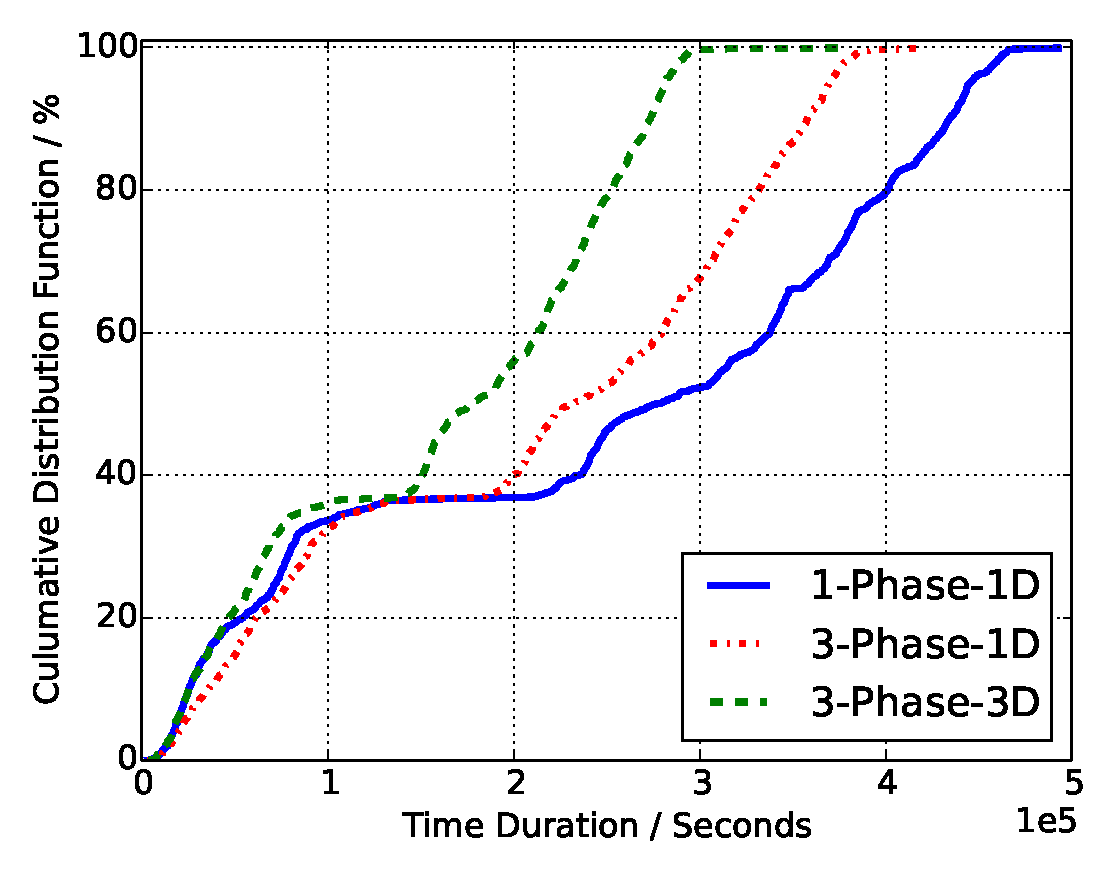
\includegraphics[width=3.2in]{3Pvs1PFigures/1000jobs_3p_vs_1p_response}
                \label{Fig:3Pvs1PResponse}
        }
        ~
        %\subfloat[Job Wait Time] {
                %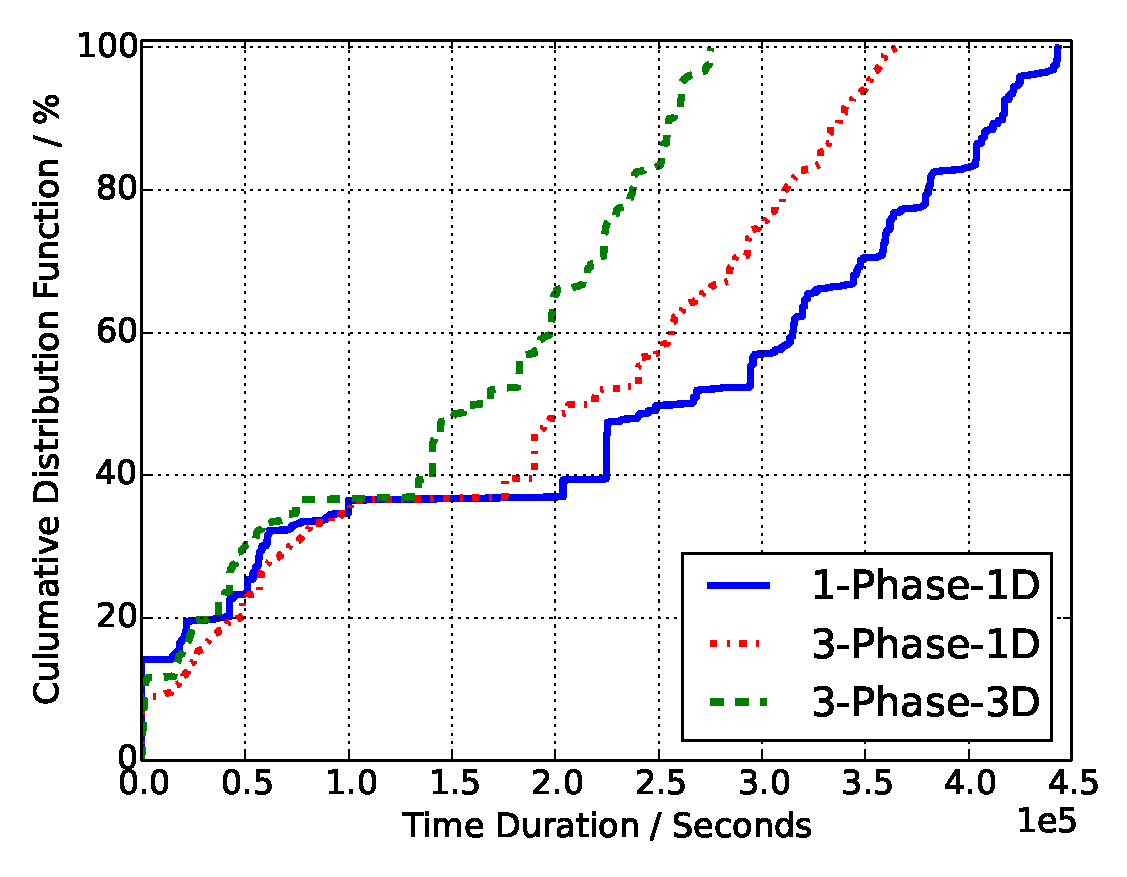
\includegraphics[width=3.2in]{3Pvs1PFigures/1000jobs_3p_vs_1p_wait}
                %\label{Fig:3Pvs1PWait}
        %}
        %\subfloat[Job Wait Input Time] {
                %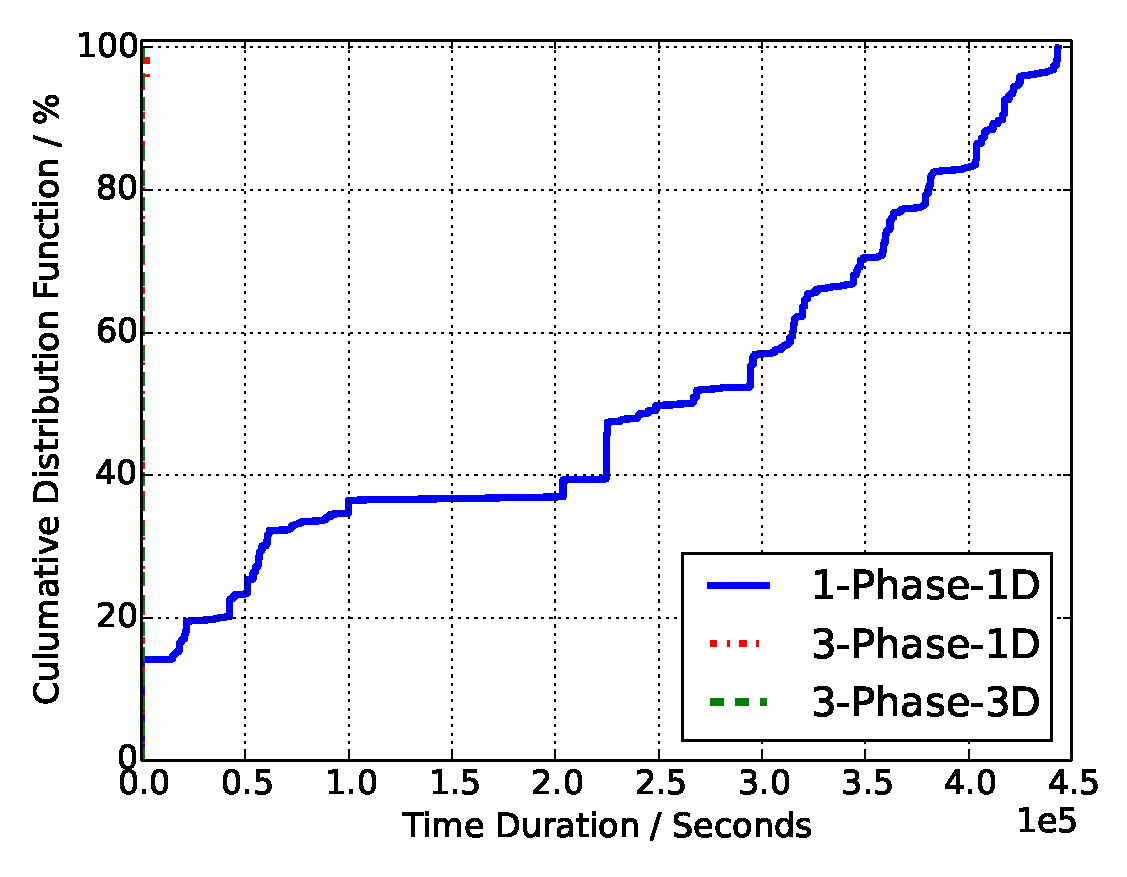
\includegraphics[width=2.3in]{3Pvs1PFigures/1000jobs_3p_vs_1p_wait_in}
                %\label{Fig:3Pvs1PWaitIn}
        %}
        %~
        \subfloat[Job Wait Run Time] {
                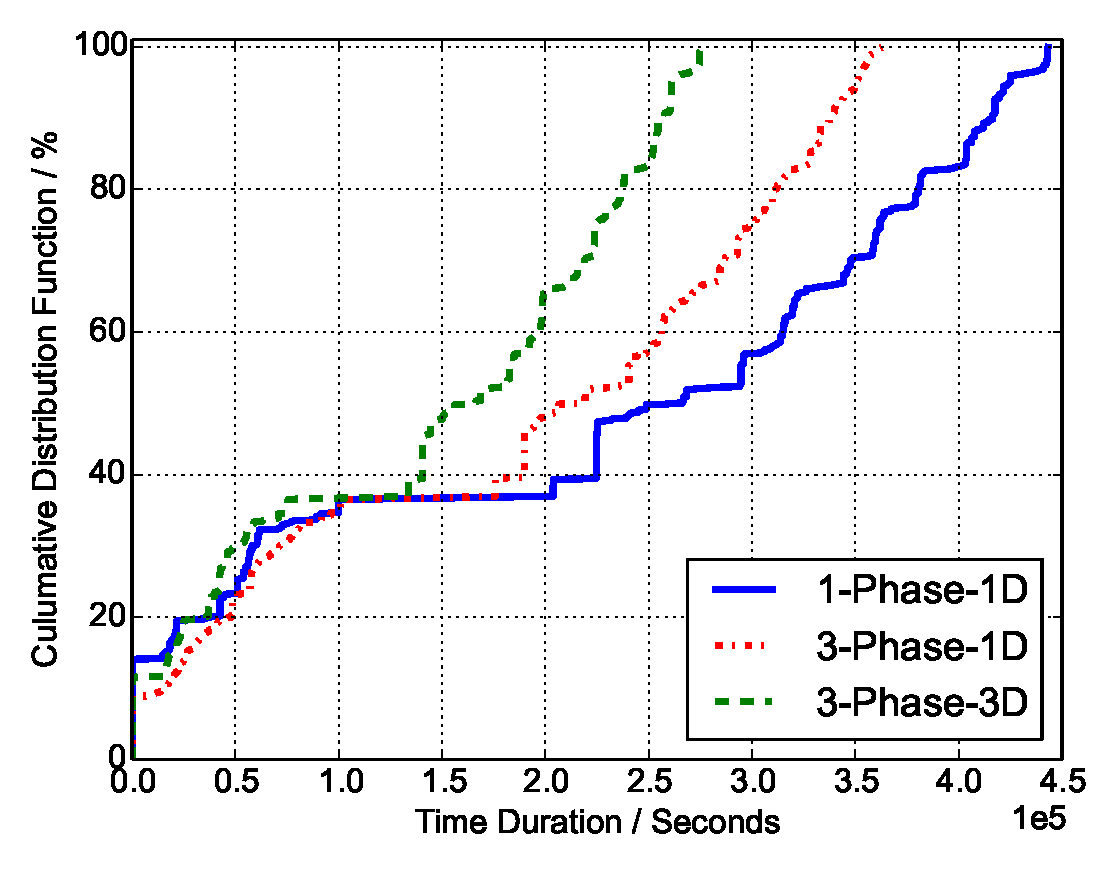
\includegraphics[width=3.2in]{3Pvs1PFigures/1000jobs_3p_vs_1p_wait_run}
                \label{Fig:3Pvs1PWaitRun}
        }
        ~
        %\subfloat[Job Wait Output Time] {
                %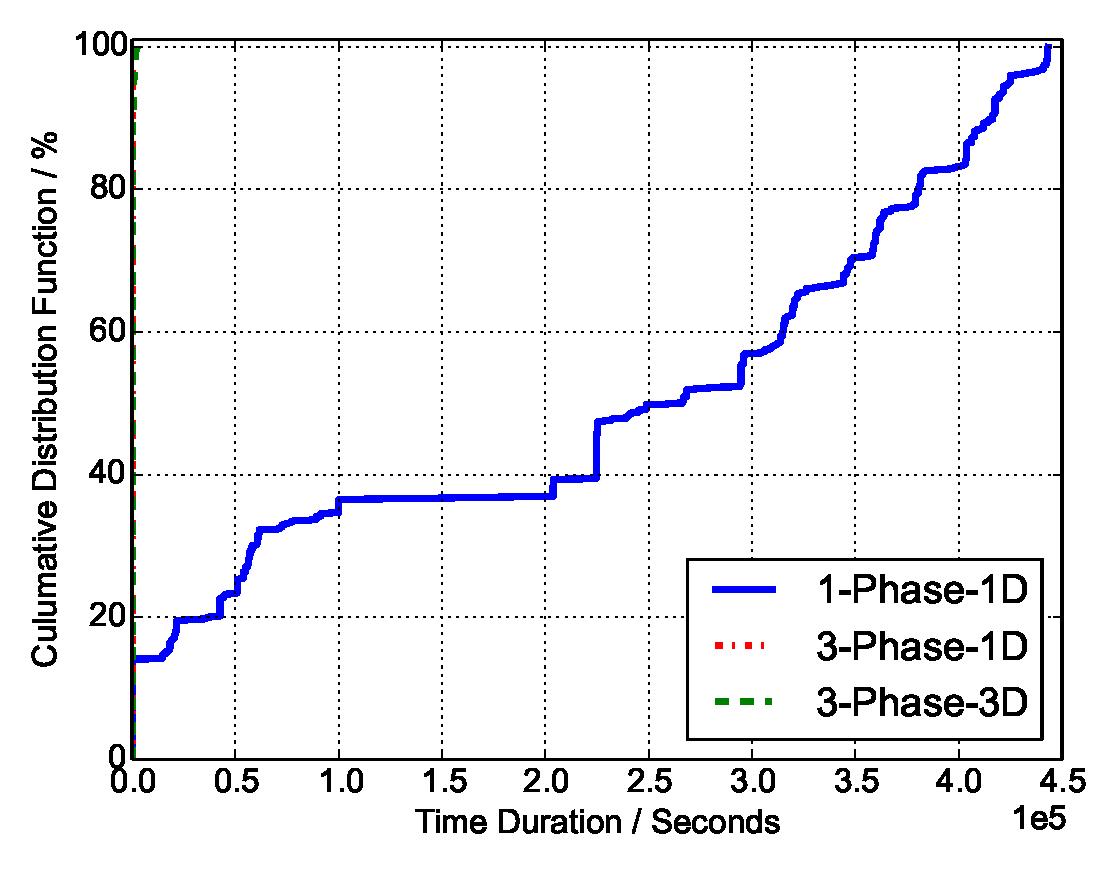
\includegraphics[width=2.3in]{3Pvs1PFigures/1000jobs_3p_vs_1p_wait_out}
                %\label{Fig:3Pvs1PWaitOut}
        %}
        \caption{Performance of 1185 Applications: 1 Phase Model vs. 3 Phase Model}
        \label{Fig:3Pvs1PPerformance}
\end{figure*}

\begin{figure*}[!t]
        \centering
        \subfloat[Job Response Time] {
                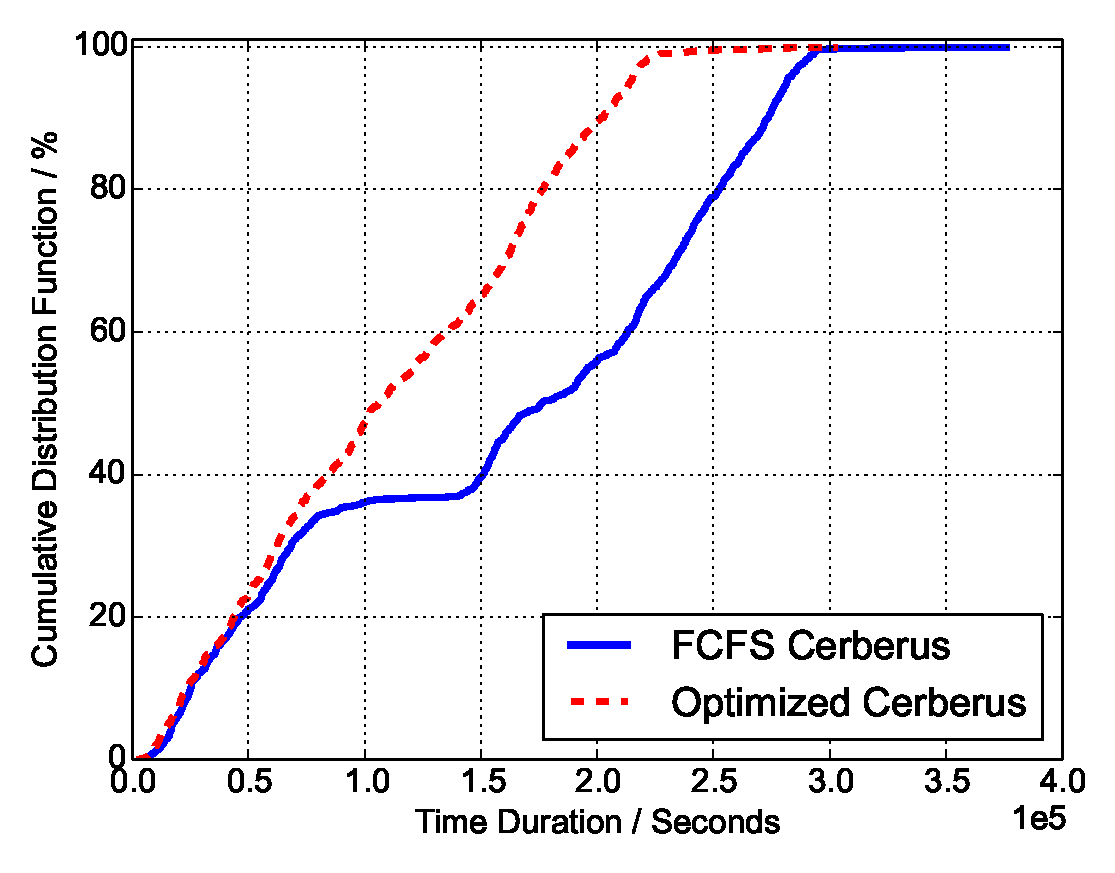
\includegraphics[width=3.2in]{DPvsFIFOFigures/1000jobs_dp_vs_fifo_response}
                \label{Fig:DPvsFIFOResponse}
        }
        ~
        \subfloat[Job Wait Run Time] {
                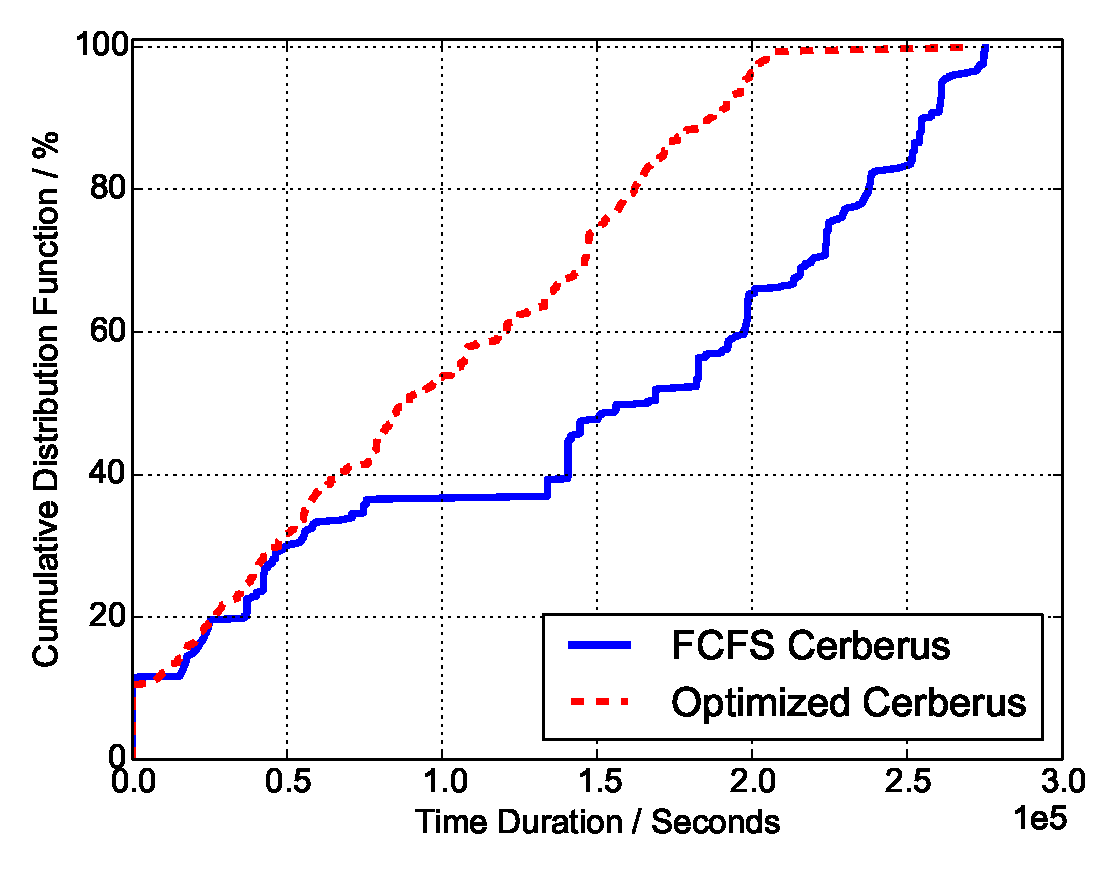
\includegraphics[width=3.2in]{DPvsFIFOFigures/1000jobs_dp_vs_fifo_wait_run}
                \label{Fig:DPvsFIFOWaitRun}
        }
        \caption{Performance of 1185 Applications: Optimized Cerberus vs. FCFS Cerberus}
        \label{Fig:DPvsFIFOPerformance}
\end{figure*}


\subsection{Q3: Cerberus vs. Optimized Cerberus}
%If we consider optimizing either burst buffer's data throughput or the parallelism across jobs,
%dynamic programming based job scheduler can further reduce jobs' wait time.
%We plot in Figure~\ref{Fig:DPvsFIFOResponse} the resulting response time of
%two versions of Cerberus:
%\begin{itemize}
%        \item \textbf{FCFS Cerberus} uses naive first come first serve policy.
%                Whoever at the front of queue are considered favorably.
%        \item \textbf{Optimized Cerberus} select these jobs in $Q_I$ and $Q_O$
%                such that volume of to be transferred data
%                is maximized by Recursion~\ref{Equ:MaxTransferDataRecursion}.
%                For jobs in $Q_R$, it chooses jobs according to the optimization solution
%                given by Equation~\ref{Equ:MaxProductRecursion}
%\end{itemize}
%As indicated by Figure~\ref{Fig:DPvsFIFOResponse}, response time of
%jobs scheduled by Optimized Cerberus is reduced.
%The most non-responsive job for Optimized Cerberus is job \#445,
%taking 303,523 seconds.
%In contrast, job \#445 takes 376,026 seconds to finish in FCFS Cerberus.
%This is 19.28\% slower than Optimized Cerberus.
%When we consider the overall response time of entire job set,
%we see more than \textit{80\% of the tasks response faster when we do optimization}.

%===========XY===============
Cerberus could deploy different optimization algorithms with regard to different
scheduling objectives.
In this section, we present the comparison of Cerberus when deploying two different 
scheduling objectives. 
The first objective is to guarantee the absolute fairness. Cerberus deploys the
naive first come first serve policy for this objective.
The other objective is to maximize the utilization in every scheduling phase. Cerberus adopts
the optimization algorithm presented in section~\ref{Sec:Scheduler}. 
In the stage-in phase, Cerberus schedules jobs in $Q_I$ and $Q_O$ according to solution given by
Recursion~\ref{Equ:MaxTransferDataRecursion}. For jobs in $Q_R$, Cerberus makes scheduling decision
based on the solution given by Recursion~\ref{Equ:MaxProductRecursion}.
We denote Cerberus coupled with two scheduling objectives 
as \textbf{FCFS Cerberus} and \textbf{Optimized Cerberus}.
\TODO{better name? FCFS and MAX-U}

As indicated by Figure~\ref{Fig:DPvsFIFOResponse}, response time of
jobs scheduled by Optimized Cerberus is reduced.
The most non-responsive job for Optimized Cerberus is job \#445,
taking 303,523 seconds.
In contrast, job \#445 takes 376,026 seconds to finish in FCFS Cerberus.
This is 19.28\% slower than Optimized Cerberus.
When we consider the overall response time of entire job set,
we see more than \textit{80\% of the tasks response faster when we do optimization}.




The time duration application waits for running,
or the time application spend in running queue,
is plotted in Figure~\ref{Fig:DPvsFIFOWaitRun}.
The tail of Optimized Cerberus shows that it holds a couple of jobs waiting
in its running queue for a very long time.
We figure out the reason of this long delay once we examine the detail of these jobs.
First they are submitted at early middle phase (Job \#435 waits 268,322 seconds).
Second, these jobs are requesting huge amount of compute nodes (163840 cores)
but comparably less burst buffer (7 TB for job \#435)
The third and the most important reason is that there are jobs requesting similarly
large number of cores but request less running time and larger amount of burst buffer.
For example, job \#434 requests 163840 cores
but its expected running time is mere 3600 seconds;
in addition, it also requests 59 TB burst buffer.
As a result, Cerberus, according to Equation~\ref{Equ:MaxProductRecursion},
favors the jobs with less request time but larger burst buffer demand.
This is interesting because it is a potential flaws in the optimization-based policy:
given the user knows the optimization objective of our scheduler,
it is possible for a user to cheat scheduler by lying about her demand.
%In other words, our optimization scheme, even though providing performance enhancement
%for the waiting time of 70\% jobs, is not strategy-proofness\cite{Ghodsi:NSDI:2011}


We can see in Figure~\ref{Fig:DPvsFIFOThroughput} the system throughput
when scheduled by Cerberus with different scheduling objectives.
For optimized Cerberus, job \#445 decides the finishing time of all 1185 jobs.
That is 303,940 seconds for Optimized Cerberus.
FCFS Cerberus makes system ends its last job, also job \#455, at 376,443 seconds.
The worst case completion improvement to FCFS-style Cerberus is 19.26\%.
When we look at the time sequence of throughput,
we found the peak value 9 jobs / 500 seconds obtained by Optimized Cerberus.
The peak throughput of FCFS Cerberus is also 9 jobs / 500 seconds.
Mean throughputs of these 3 scheduling methods are drawn
as bar chart in Figure~\ref{Fig:DPvsFIFOThroughput}.
\textit{Comparing with FCFS Cerberus, Optimized Cerberus achieves
23.87\% higher average throughput (1.951 jobs / 500 seconds).}

\begin{figure}[!t]
        \centering
        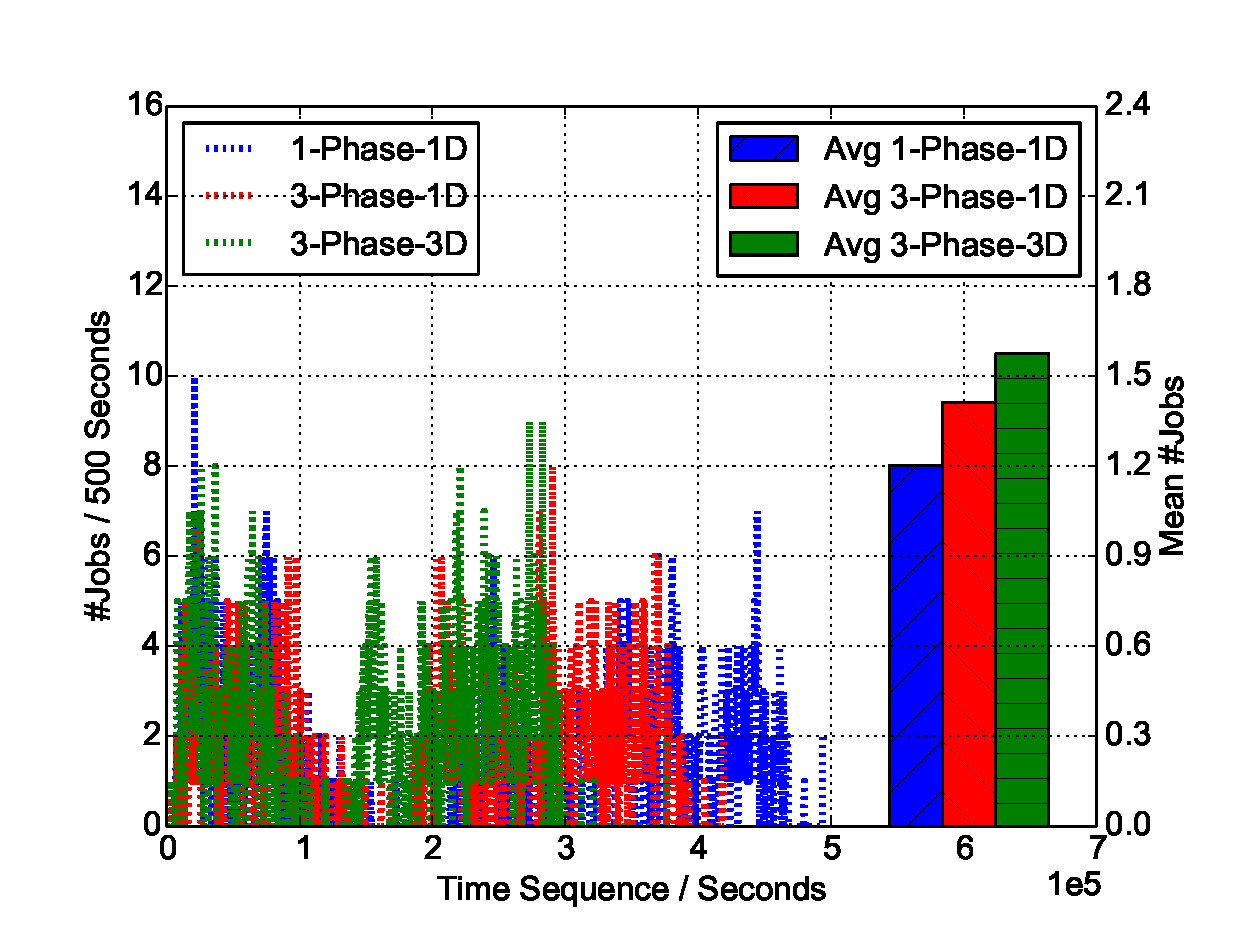
\includegraphics[width=3.2in]{3Pvs1PFigures/1000jobs_3p_vs_1p_throughput}
        \caption{System Throughput, 1 Phase Model vs. 3 Phase Model}
        \label{Fig:3Pvs1PThroughput}
\end{figure}


\begin{figure}[!t]
        \centering
        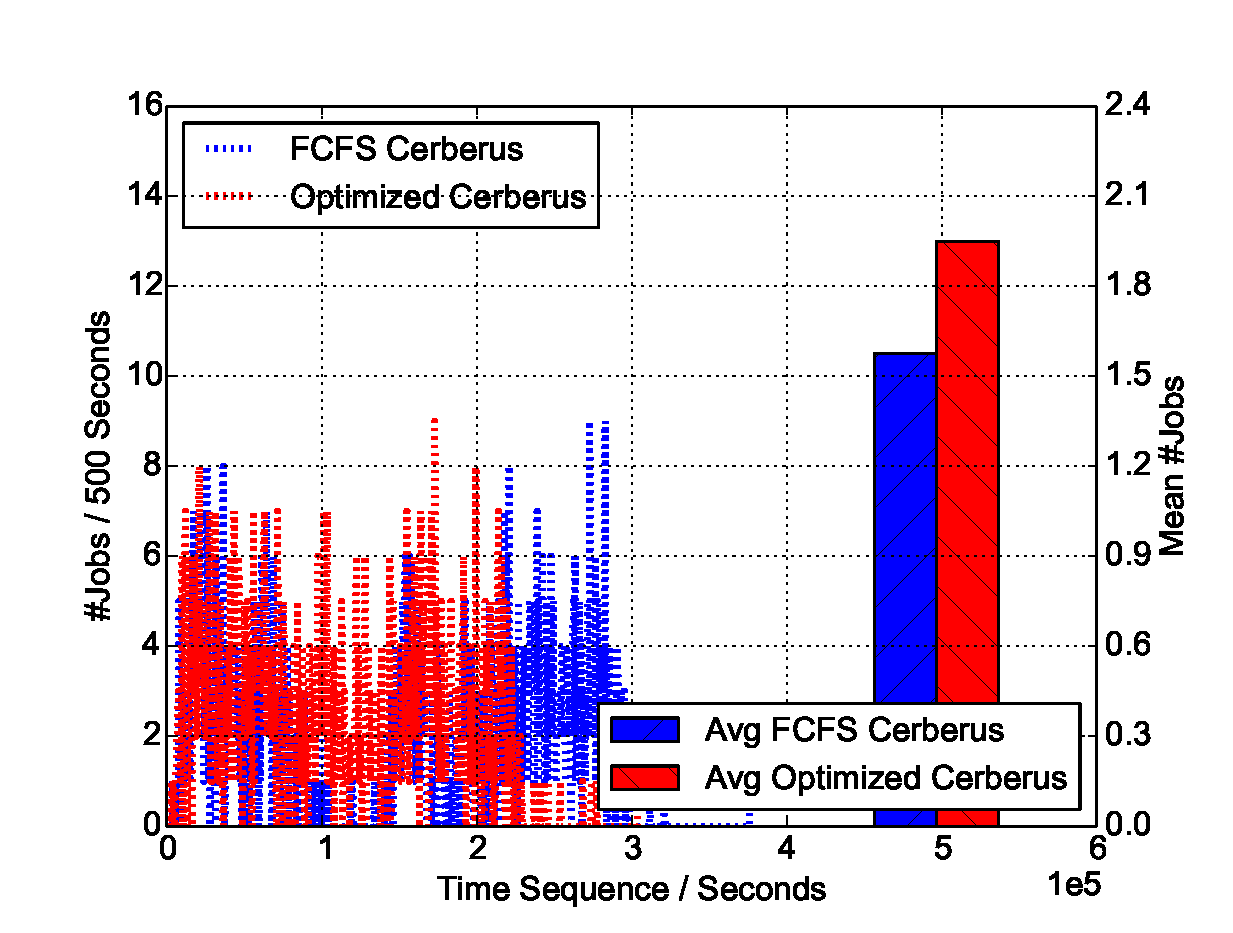
\includegraphics[width=3.2in]{DPvsFIFOFigures/1000jobs_dp_vs_fifo_throughput}
        \caption{System Throughput, Optimized Cerberus vs. FCFS Cerberus}
        \label{Fig:DPvsFIFOThroughput}
\end{figure}


%Table~\ref{Tab:OptimizationTime} demonstrate that 
Our dynamic programming based optimized Cerberus can schedule jobs online,
even though solving the optimization problem is theoretically NP-hard.
For Optimized Cerberus, it solved about 8400 Problems~\ref{Equ:MaxTransferData} and
Problem~\ref{Equ:MaxProduct} when scheduling all the jobs in workload,
taking less than 370 seconds.
The time overhead of solving each optimization is about 0.04 seconds per time.

%\begin{table}[!t] 
        %\renewcommand{\arraystretch}{1.3}
        %\caption{Time Consumption in Dynamic Programming}
        %\label{Tab:OptimizationTime}
        %\centering
        %\begin{tabular}{l|c}
                %\hline
                %Optimization Policy Used & Optimized Cerberus\\
                %\hline
                %\hline
                %Simulation Run Time / seconds & 375.55\\
                %Optimization Run Time / seconds & 364.62\\
                %Total Number of Optimizations & 8406\\
                %\hline
        %\end{tabular}
%\end{table}





\section{Related Works}
\label{Sec:RelatedWorks}

I/O contention in HPC systems draws a lot of attension in the community because it is one of the major culprits for parallel applications’ performance variability \cite{hashimoto:ICNC:2012} \cite{dorier:IPDPS:2014} \cite{yildiz:IPDPS:2016}


Hashimoto et al. evaluate the performance variability of each job when they run concurrently on the same physical computing server. They identify that network I/O sharing introduces most of the performance degradation \cite{hashimoto:ICNC:2012}.  
Dorier et al. analyze the I/O interference between two applications. They make quantified study about performance improvement obtained by interrupting or delaying either one in order to avoid I/O contention \cite{dorier:IPDPS:2014}.
Yildiz et al. \cite{yildiz:IPDPS:2016} explore the various root causes of I/O interference in HPC storage systems. They find that in many situations interference is a result of bad flow control in the I/O path, rather than being caused by some single bottleneck in one of its components.

The solutions for alleviate I/O contention between concurrently running jobs have been proposed in recent works \cite{lofstead:sc:2010} \cite{zhou:Cluster:2015} \cite{SlurmBBGuide} \cite{Liu:MSST:2012}.
Lofstead et al. schedule each application’s I/O request individually without a global view from system’s perspective. Their solutions require supports from specific I/O management in the system level for better results \cite{lofstead:sc:2010}. 
Zhou et al. design a new I/O aware batch scheduler to address the I/O contention problem at batch scheduling level. The new scheduler schedules and coordinates the I/O requrests without hurting the fairness across applications \cite{zhou:Cluster:2015}. 
Liu et al. proposed to move many file handling to the I/O nodes to ameliorate the I/O pressure from the massive number of compute nodes \cite{Liu:MSST:2012}.
Slurm developed a new module for its batch scheduler that could allocate burst buffer resource to submitted user jobs. With pre-allocated burst buffer, I/O performance of user job can be greatly improved \cite{SlurmBBGuide} However, the way they do the resource allocation is in first-come, first-serve manner without any optimizatoin. 

Our work is different from the existing research in the following ways. In our novel scheduling framework, user job can require burst buffer resource for improving its I/O operation. Job being characterized into three phases based on their I/O operation and our new scheduler, Cerberus, makes scheduling decisions for each specific phases. Cerberus is also integrated with different optimizatoin algorithms for the objectives of maximizing resource utilization and system throughput.


% \cite{SlurmBBGuide}




\section{Conclusion and Future Work}
\label{Sec:Conclusion}

We explore how the batch scheduler can efficiently allocate burst buffer to absorb three general types of IO operations:
data staging in, application checkpointing, and data staging out.
We propose a three-phase job model which is tailored to burst buffer's typical use cases.
Burst-buffer-aware Cerberus is developed on the basis of the three-phase job model.
We divide the scheduling problem into three sub-phases, and conquer them independently using dynamic programming based optimization.
Simulation results show that Cerberus significantly improves both the application-level and the system-level performance.

%Since the burst buffer enabled system is not ready for the massive 
%use by the community, 
%there is no study about the burst buffer demand of the typical scientific workloads.
We plan to study the optimal workload scheduling in Cerberus with diverse resource demands,
which would provide useful insight for computing facilities to configure their burst buffer subsystems.
We will also integrate optimization algorithms to Cerberus to satisfy various scheduling objectives.
We also plan to make Cerberus more versatile to deal with new schedulable system resources.




% An example of a floating figure using the graphicx package.
% Note that \label must occur AFTER (or within) \caption.
% For figures, \caption should occur after the \includegraphics.
% Note that IEEEtran v1.7 and later has special internal code that
% is designed to preserve the operation of \label within \caption
% even when the captionsoff option is in effect. However, because
% of issues like this, it may be the safest practice to put all your
% \label just after \caption rather than within \caption{}.
%
% Reminder: the "draftcls" or "draftclsnofoot", not "draft", class
% option should be used if it is desired that the figures are to be
% displayed while in draft mode.
%
%\begin{figure}[!t]
%\centering
%\includegraphics[width=2.5in]{myfigure}
% where an .eps filename suffix will be assumed under latex, 
% and a .pdf suffix will be assumed for pdflatex; or what has been declared
% via \DeclareGraphicsExtensions.
%\caption{Simulation results for the network.}
%\label{fig_sim}
%\end{figure}

% Note that the IEEE typically puts floats only at the top, even when this
% results in a large percentage of a column being occupied by floats.


% An example of a double column floating figure using two subfigures.
% (The subfig.sty package must be loaded for this to work.)
% The subfigure \label commands are set within each subfloat command,
% and the \label for the overall figure must come after \caption.
% \hfil is used as a separator to get equal spacing.
% Watch out that the combined width of all the subfigures on a 
% line do not exceed the text width or a line break will occur.
%
%\begin{figure*}[!t]
%\centering
%\subfloat[Case I]{\includegraphics[width=2.5in]{box}%
%\label{fig_first_case}}
%\hfil
%\subfloat[Case II]{\includegraphics[width=2.5in]{box}%
%\label{fig_second_case}}
%\caption{Simulation results for the network.}
%\label{fig_sim}
%\end{figure*}
%
% Note that often IEEE papers with subfigures do not employ subfigure
% captions (using the optional argument to \subfloat[]), but instead will
% reference/describe all of them (a), (b), etc., within the main caption.
% Be aware that for subfig.sty to generate the (a), (b), etc., subfigure
% labels, the optional argument to \subfloat must be present. If a
% subcaption is not desired, just leave its contents blank,
% e.g., \subfloat[].


% An example of a floating table. Note that, for IEEE style tables, the
% \caption command should come BEFORE the table and, given that table
% captions serve much like titles, are usually capitalized except for words
% such as a, an, and, as, at, but, by, for, in, nor, of, on, or, the, to
% and up, which are usually not capitalized unless they are the first or
% last word of the caption. Table text will default to \footnotesize as
% the IEEE normally uses this smaller font for tables.
% The \label must come after \caption as always.
%
%\begin{table}[!t]
%% increase table row spacing, adjust to taste
%\renewcommand{\arraystretch}{1.3}
% if using array.sty, it might be a good idea to tweak the value of
% \extrarowheight as needed to properly center the text within the cells
%\caption{An Example of a Table}
%\label{table_example}
%\centering
%% Some packages, such as MDW tools, offer better commands for making tables
%% than the plain LaTeX2e tabular which is used here.
%\begin{tabular}{|c||c|}
%\hline
%One & Two\\
%\hline
%Three & Four\\
%\hline
%\end{tabular}
%\end{table}


% Note that the IEEE does not put floats in the very first column
% - or typically anywhere on the first page for that matter. Also,
% in-text middle ("here") positioning is typically not used, but it
% is allowed and encouraged for Computer Society conferences (but
% not Computer Society journals). Most IEEE journals/conferences use
% top floats exclusively. 
% Note that, LaTeX2e, unlike IEEE journals/conferences, places
% footnotes above bottom floats. This can be corrected via the
% \fnbelowfloat command of the stfloats package.



% conference papers do not normally have an appendix


% use section* for acknowledgment
\ifCLASSOPTIONcompsoc
  % The Computer Society usually uses the plural form
  \section*{Acknowledgments}
\else
  % regular IEEE prefers the singular form
  \section*{Acknowledgment}
\fi


The authors would like to thank...



% trigger a \newpage just before the given reference
% number - used to balance the columns on the last page
% adjust value as needed - may need to be readjusted if
% the document is modified later
%\IEEEtriggeratref{8}
% The "triggered" command can be changed if desired:
%\IEEEtriggercmd{\enlargethispage{-5in}}

% references section

% can use a bibliography generated by BibTeX as a .bbl file
% BibTeX documentation can be easily obtained at:
% http://mirror.ctan.org/biblio/bibtex/contrib/doc/
% The IEEEtran BibTeX style support page is at:
% http://www.michaelshell.org/tex/ieeetran/bibtex/
\bibliographystyle{IEEEtran}
% argument is your BibTeX string definitions and bibliography database(s)
\bibliography{IEEEabrv,ref}
%
% <OR> manually copy in the resultant .bbl file
% set second argument of \begin to the number of references
% (used to reserve space for the reference number labels box)
%\begin{thebibliography}{1}

%\bibitem{IEEEhowto:kopka}
%H.~Kopka and P.~W. Daly, \emph{A Guide to \LaTeX}, 3rd~ed.\hskip 1em plus
  %0.5em minus 0.4em\relax Harlow, England: Addison-Wesley, 1999.

%\end{thebibliography}




% that's all folks
\end{document}


